\documentclass[11pt,  oneside, openany]{book}
\usepackage[greek, italian]{babel}
\usepackage{geometry}
\usepackage{float}
\usepackage{graphicx} 
\usepackage{amsmath}
\usepackage{subfig}
\usepackage{array}
\usepackage{amsfonts}
\usepackage{multirow}
\geometry{a4paper} 
\usepackage{listings} % necessario per inclusione codice sorgente
\usepackage{color} % syntax highlighting
\usepackage{url}
\usepackage{pdfpages}
\usepackage{caption}


\newcommand{\source}[1]{\caption*{Fonte: {#1}} }

% \textit {f}  
% ~, `` ''
% Controllare poi che i capitoli e paragrafi citati siano corretti. (es vedi Capitolo 4)

\pdfinfo{
   /Author (Rita Folisi)
   /Title  (Elaborato finale)
 
}

\title{Elaborato finale}
\date{}
\author{Rita Folisi}

\begin{document}
	\pagenumbering{gobble}

  \begin{titlepage}
    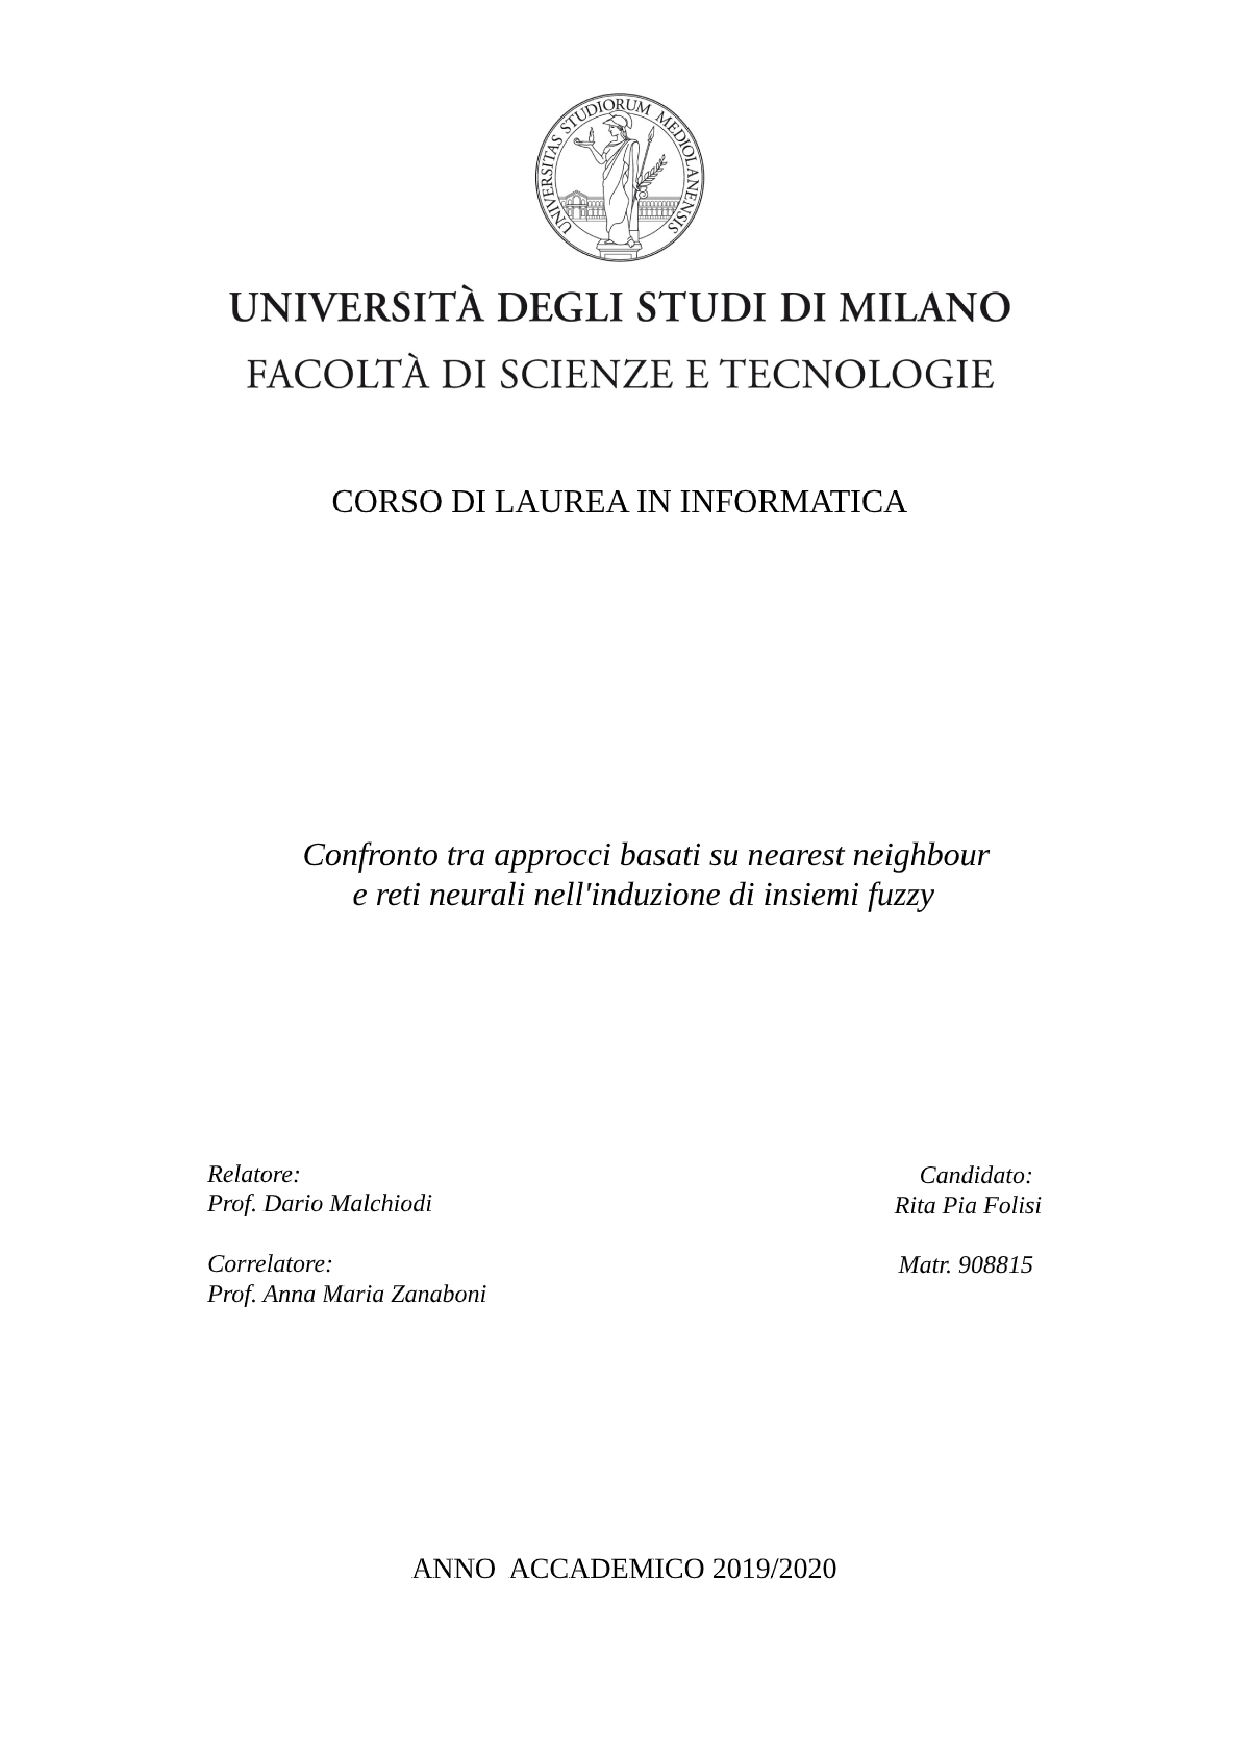
\includepdf{Immagini/Frontespizio.pdf}
    \thispagestyle{empty}
  \end{titlepage}



	\pagenumbering{arabic}

	\chapter*{Ringraziamenti}
Ho intrapreso questo percorso universitario fresca di diploma classico e incuriosita da un mondo in apparenza opposto a ciò a cui mi ero sempre interfacciata. Sono stati tre anni pieni di dubbi, ma anche di tante soddisfazioni. Ho imparato come trovare un po' di filosofia e di creatività anche in materie prettamente scientifiche. Ho constatato attivamente come ogni campo sia intrinsicamente connesso con tutti gli altri. Sono cresciuta e ho irrimediabilmente esteso la mia visione del mondo. Per questo motivo, il mio primo ringraziamento è rivolto ai professori incontrati durante questo percorso, da cui sento di aver imparato molto. Ringrazio, in particolare, il mio relatore e la mia correlatrice, Dario Malchiodi e Anna Maria Zanaboni, per avermi fatto scoprire questo campo molto stimolante, per il supporto e per il sostegno continuo durante tutto il percorso. Un sentito grazie sicuramente alla mia compagna di tirocinio, Alessia, che ho avuto modo di conoscere meglio in questi mesi. Ti ringrazio tantissimo per aver condiviso tutto, dalle soddisfazioni di un codice funzionante al primo colpo ai più grandi scleri in chiamata. Spero di poter lavorare di nuovo con te! 

Ringrazio tutte le persone che ho incontrato in questo percorso che in un qualche modo mi hanno regalato qualcosa. Ringrazio Lisa e Pietro per l'incessante supporto e per aver sempre creduto nelle mie capacità, anche quando io stessa non ci riuscivo. Ringrazio le pecorelle per le tante giornate di studio insieme. Ringrazio Patrizio per l'instancabile supporto davanti a ogni difficoltà, per avermi incoraggiato a dare sempre del meglio, senza cedere alle insicurezze. 

Ringrazio infine la mia famiglia per avermi permesso di intraprendere questo percorso e per avermi sostenuto, anche laddove era più difficile farlo. Un grandissimo e fortissimo grazie a mia sorella, per la sua grande pazienza e per trovare una nota positiva anche nelle giornate peggiori. 


    \tableofcontents

	\chapter*{Introduzione}
In questo elaborato si descrive il tirocinio, effettuato presso l'Università degli Studi di Milano, che riguarda la ricerca, la modifica e il riuso di algoritmi per l'induzione della funzione di appartenenza a insiemi fuzzy. 

Nell'ambito dell'apprendimento automatico, una classe di problemi che ha assunto grande rilevanza è legata alla classificazione: dato un oggetto, ci si aspetta che si riesca a predire la sua classe di appartenenza. Esistono vari approcci al problema, ognuno dei quali con i propri punti di forza e di debolezza. Nel tirocinio ci si è occupati di insiemi fuzzy, dal momento che riescono a cogliere l'ambiguità caratterizzante il linguaggio naturale, consentendo una maggiore flessibilità nella classificazione stessa. Nell'ambito degli insiemi fuzzy, fondamentale è il concetto di funzione di appartenenza, che definisce il grado con cui un dato oggetto può appartenere a una classe. Ricoprendo valori da 0 a 1, la funzione di appartenenza riesce così a sintetizzare anche la parziale appartenenza di un oggetto a una data classe, superando il binarismo della logica classica. 

In letteratura sono stati presentati molteplici modi per poter indurre la funzione di appartenenza. Nel tirocinio sono stati esaminati algoritmi basati sulle reti neurali e sul k-Nearest Neighbour, illustrandone inoltre le principali varianti. In particolare, è stato implementato un algoritmo per ogni famiglia: per le reti neurali ci si è soffermati sul Fuzzy min-max Neural Network, mentre per il k-Nearest Neighbour è stato analizzato il Fuzzy k-Nearest Neighbour. Per entrambi gli algoritmi si è partiti da codice preesistente sul quale sono state attuate modifiche per poter in seguito effettuare esperimenti e valutare le prestazioni. Gli algoritmi sono stati valutati sui dataset Iris e Breast-Cancer, ottenendo dei buoni risultati. Il Fuzzy min-max classifica i dati con un'accuratezza maggiore e impiega meno tempo a elaborarli e a effettuare predizioni; il Fuzzy k-Nearest Neighbour, invece, fornisce un errore minore nell'indurre i gradi di appartenenza. 

L'elaborato è strutturato come segue: nel Capitolo 1 sono introdotte le tematiche relative all'apprendimento automatico e logica fuzzy, illustrando il problema sul quale l'elaborato si concentra. Nel Capitolo 2 si passano in rassegna i concetti di reti neurali e di k-Nearest Neighbour, per illustrarne il funzionamento e fornire una panoramica delle possibili varianti. Nel Capitolo 3 viene infine descritta l'implementazione e si forniscono i risultati degli esperimenti effettuati, sotto forma di tabelle e grafici. 

	\chapter{Apprendimento automatico e logica fuzzy}
Nel seguente capitolo si passano in rassegna i concetti di apprendimento automatico e di logica fuzzy, illustrando come i due argomenti possano essere coniugati insieme. Nel Paragrafo 1.1 ci si soffermerà sull'apprendimento supervisionato, di cui i metodi proposti in seguito faranno parte. Nel Paragrafo 1.2 si riprenderanno i concetti relativi ai \textit {fuzzy set}, fino a illustrare cosa significa indurne la funzione di appartenenza. 

	\section{Apprendimento supervisionato}

Con apprendimento automatico si intende l'abilità di una macchina di apprendere in maniera autonoma a partire da dati o da osservazioni, attraverso diversi algoritmi. A partire da questi dati la macchina impara una funzione, che permette di risolvere generiche istanze di un fissato problema. Nel seguito, sarà utilizzato il termine ``esempio'' per riferirsi ai dati sopracitati. In genere, vengono considerate varie classi di problemi, quali la classificazione, la regressione e il clustering. 

Da un punto di vista formale~\cite {mlstanford} si considerino un problema di riferimento, delle istanze di un problema e una funzione  $f$, che codifica la soluzione delle istanze del problema. Le istanze del problema sono descritte da un vettore  $X$ = $x_1...x_n$ composto da $n$ elementi e sono associate tramite la funzione $f$ ognuna alla propria soluzione. La funzione $f$ non è nota, ma si utilizza una funzione $h$ che la approssima al meglio\footnote{`E bene precisare che la bontà di tale approssimazione è legata alla metrica, la cui scelta non è una questione banale, come si vedrà in seguito}.  Le funzioni \textit {f} e \textit {h} sono definite sul vettore $X$ descritto precedentemente. Viene assunto a priori che \textit {h} viene selezionata da una classe di funzioni \textit {H}, alla quale \textit {f} può appartenere.  All'interno della classe di funzioni, \textit {h} viene scelta in base a $\Xi$, un insieme contenente $m$ esempi di apprendimento. Una volta scelta, \textit {h} viene implementata da una macchina, che avrà dunque input X e in output \textit {h}(X). 

L'apprendimento automatico può essere principalmente di due tipi: si parla, infatti, di modalità supervisionata e non supervisionata. In questo elaborato, tuttavia, verrà trattato soltanto l'apprendimento supervisionato, in cui l'insieme $\Xi$ contiene le coppie input-output della funzione \textit {f}. 
Se il processo di apprendimento riesce a selezionare una funzione \textit {h} che approssima bene \textit {f} per i valori di $\Xi$, allora si può ipotizzare che \textit {h} sia un'ottima approssimazione per \textit {f} anche in generale. In altri termini, attraverso esempi di apprendimento costituiti da coppie di input e di output, viene costruito il modello, cioè una funzione capace di fornire buone predizioni in relazione a nuovi input. 
Quando tale output è rappresentato da una variabile discreta si parla di classificazione, se invece è una variabile continua si parla di regressione. Il campo esaminato durante il tirocinio riguarda i problemi di classificazione e pertanto l'obiettivo dei metodi presentati in seguito sarà, dato un vettore di input, fornire una predizione sperabilmente corretta. Gli output possono anche essere definiti come $label$ o etichetta. D'altra parte, il vettore di input $X$ può essere definito anche come \textit {feature vector} e le componenti $x_i$ \textit come {feature} o attributi, i cui valori possono essere di tre tipologie: numeri reali, discreti o valori categorici.
Un esempio di problema di classificazione è il filtraggio anti-spam. In questo caso, gli esempi di addestramento hanno come vettore $X$  il contenuto testuale e i metadati di ogni mail, mentre come etichetta un bit che dichiara se il messaggio sia spam o meno.

Una volta addestrato il modello con gli esempi di apprendimento, occorre valutare le performance per comprendere se questo è in grado di eseguire correttamente il suo compito. In funzione del problema da affrontare, si adottano criteri diversi: nel caso della classificazione si utilizza in genere l'accuratezza, mentre nella regressione si  usano funzioni di errore. L'accuratezza è il numero di predizioni corrette divise per il totale delle predizioni effettuate e viene espresso in percentuale. 

Tra le funzioni di errore, è molto comune l'errore quadratico medio (\textit{mean square error}), che quantifica quanto le predizioni eseguite dal modello siano vicine all'etichetta attraverso questa formula: 

$$MSE = \frac{1}{n}\sum_{i=1}^{n}(y_{i} - h(x_{i}))^{2}$$ 
dove $y_i$ è l'etichetta, mentre $h(x_{i})$ è la predizione effettuata dal modello. 
Un'altra funzione di errore utilizzata è RMSE ovvero la radice quadrata dell'errore quadratico medio: 

$$RMSE = \sqrt{\frac{1}{n}\sum_{i=1}^{n}(y_{i} - h(x_{i}))^{2}}$$. 

In genere, alla funzione di errore si affianca anche una soglia, che precisa quale il margine di errore è considerato accettabile. Le funzioni di errore in realtà  possono essere utilizzate anche con problemi di classificazione, ma l'accuratezza non viene utilizzata mai con problemi di regressione. 
La valutazione non viene effettuata sugli esempi utilizzati per l'apprendimento, dal momento che l'obiettivo del modello è generalizzare con dati diversi da quelli osservati in precedenza. Dati degli esempi del problema che si vuole risolvere, occorre distinguere una parte di dati dedita ad addestrare il modello (\textit{training set}) e un'altra dedita a valutarne la prestazione (\textit{testing set}). Il primo verrà utilizzato in fase di apprendimento, mentre il secondo verrà utilizzato esclusivamente alla fine per decretare le performance del modello. I due set possono presentare delle criticità tali da poter alterare l'intero processo di apprendimento e valutazione. Ad esempio, possono avere una dimensione molto elevata di feature, comportando un aumento della complessità computazionale dell'algoritmo di apprendimento; per risolvere questo problema, si utilizzano algoritmi di selezione delle feature, con lo scopo di selezionare quelle più rilevanti per migliorare le predizioni e le performance generali. Un'altra criticità è causata dal rumore nei dati. Nel caso sia presente nei dati di training, il rumore di classe altera i valori di \textit{f}, mentre il rumore di attributo altera i valori delle componenti dei vettori di input, compromettendo dunque la corretta associazione input-output. Inoltre, è bene osservare quanto il training set sia rappresentativo del campo in analisi: infatti, può accadere che questo presenti poca varietà e che il metodo dunque non sia in grado di generalizzare. Ad esempio, se nel training set sono presenti, sotto la label di ``orologio'', solo immagini di orologi rotondi e di color rosso, quando il modello si ritroverà a dover predire la label di un orologio quadrato e giallo probabilmente non darà la risposta corretta. Questo fenomeno prende il nome di \textit {overfitting} ed è facilmente visibile quando il modello si adatta molto ai dati di training ma riporta performance sensibilmente inferiori con i dati di testing. 

\begin{figure}[h!]
\begin{center}
  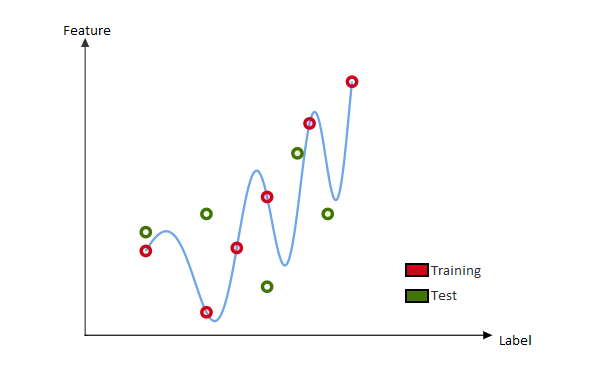
\includegraphics[width=13cm]{Immagini/Overfitting.png}\\
  \caption{Illustrazione grafica del fenomeno dell'overfitting}
\end{center}
\end{figure}

Graficamente, si avrà la situazione presente in Figura 1.1, ovvero la funzione in blu $h$, appresa dal modello, si adatterà perfettamente ai dati di training (segnati in rosso), ma non riuscirà a predire bene i dati di testing. In altri termini, se il modello allenato viene eseguito sui dati di training, il modello produrrà un numero sensibilmente minore di errori rispetto a quando viene eseguito sui dati di testing. Un overfitting può essere causato anche da una suddivisione casuale dei dati che comporti l'inserimento nel training set di osservazioni non generali. Più in generale, nel valutare le performance, è bene considerare quanto la scelta di determinati esempi di apprendimento possa influenzare le performance. Può infatti succedere che una buona valutazione sia data da una scelta fortuita di esempi di apprendimento, mentre con un'altra scelta di esempi tale modello non dia la stessa performance. Dunque la valutazione effettuata dopo aver allenato il modello è la valutazione di un solo esperimento, non per forza del modello in sé. Occorre dunque uno strumento che possa generalizzare le valutazioni delle performance complessive di un modello. Per la risoluzione del problema, si rimanda ai paragrafi successivi. 


Normalmente, prima di effettuare il processo di apprendimento, occorre impostare uno o più iperparametri. Si definiscono iperparametri tutte le parti del modello da impostare prima di iniziare la fase di apprendimento, mentre i parametri sono quelle parti del modello apprese durante la fase di apprendimento. Impostare gli iperparametri non è un'operazione semplice, dal momento che una configurazione erronea può incidere notevolmente sulle performance del modello. Si parla pertanto di \textit{model selection} (selezione del modello) o \textit{tuning degli iperparametri}, che si servono di un sottinsieme del training set, che prende il nome di \textit{validation set}. L'obiettivo è trovare la combinazione di iperparametri che ottimizza le performance del modello. Si definiscono gli insiemi di valori potenziali di ogni iperparametro e il modello viene addestrato con tutte le combinazioni possibili. Si decreta poi il \textit{validation score} (punteggio di validazione), che è coerente con il criterio scelto per valutare le performance del modello alla fine. Infine, si selezionano i valori che massimizzano il validation score e vengono assegnati agli iperparametri del modello. 
 

Per risolvere il problema della model selection e della generalizzazione delle valutazioni, si ricorre alla \textit{k-fold cross validation}. Più in generale, la cross validation è una tecnica utilizzata per la suddivisione del dataset in training set e in validation set nel primo caso o in training set e in testing set nel secondo caso. Si prenda ad esempio il problema della model selection e quindi della suddivisione in training set e in validation set. Si definisce il numero di fold \textit{k} e si divide il dataset $\Xi$ in \textit{k} sottinsiemi mutuamente esclusivi e di ugual dimensione: $\Xi_1 ... \Xi_k$. In seguito, si reitera l'algoritmo di apprendimento \textit{k} volte considerando a ogni iterazione il sottinsieme $\Xi_k$ come training set e i rimanenti come validation set. La valutazione finale viene effettuata facendo la media delle valutazioni parziali dei sottinsiemi. In Figura 1.2 è presente una visualizzazione grafica della cross validation, con suddivisione in training set e validation set. Tale procedimento è del tutto analogo anche nel caso in cui si voglia generalizzare le valutazioni delle performance e dunque suddividere in training set e testing set. Qualora si volesse risolvere in maniera combinata entrambi i problemi, sarà necessario fare una crossvalidation annidata nell'altra. Per maggiori dettagli implementativi si rimanda al Capitolo 3. 

\begin{figure}[h!]
\begin{center}
  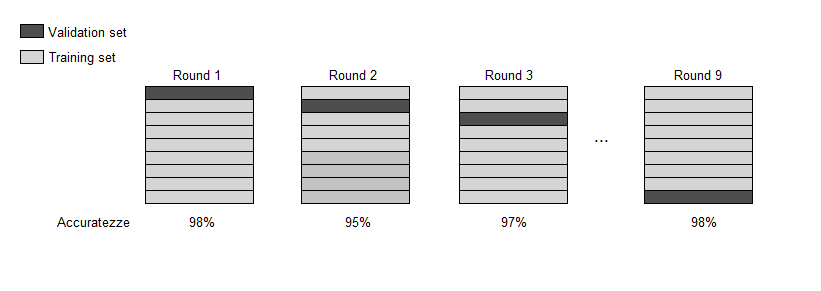
\includegraphics[width=13cm]{Immagini/Crossvalidation.png}\\
  \caption{Cross validation}
\end{center}
\end{figure}

	\section{Logica fuzzy e fuzzy set}
Il linguaggio e il ragionamento umano, spesso imprecisi e complessi, difficilmente sono colti appieno dalla logica classica basata sull'assegnazione di un valore di verità binario (vero o falso). Infatti, nel linguaggio naturale, molte espressioni risultano ambigue e, per la loro mancanza di formalità, diventano difficilmente trattabili con i classici strumenti della matematica. Una proposizione, in particolare, viene definita imprecisa nel momento in cui contiene predicati che possono essere veri o falsi solo parzialmente o solo a un certo grado. Un esempio concreto è la frase ``Il caffè è abbastanza dolce''. In questa frase il concetto di dolce non è formalizzato e non ha un significato fisso, in quanto non viene indicata una certa quantità di zucchero affinché il caffè possa considerarsi effettivamente dolce. Inoltre, è accompagnata dall'avverbio ``abbastanza'', che non esprime a sua volta un grado di certezza ben definito. Pertanto, alla proposizione è impossibile affidare un valore di verità binario, dal momento che il grado di dolcezza è soggettivo e, dunque, non interpretabile universalmente. Per poter trattare queste situazioni si introduce la \textit{logica fuzzy}~\cite{fuzzylogicintro}, un'estensione della logica booleana. La logica fuzzy attribuisce a ogni proposizione un valore di verità compreso tra 0 e 1, estremi inclusi: pertanto, è capace di trattare proposizioni vere (valore pari ad 1), false (valore pari a 0) e parzialmente vere o false (valore compreso tra 0 e 1). Permettendo quindi alle proposizioni di trovarsi in uno stato diverso dal vero o falso, la logica fuzzy consente di descrivere con flessibilità il ragionamento umano e gestire l'incertezza e l'inesattezza. Per questo motivo è ampiamente utilizzata in molti domini di applicazione, come processi decisionali, analisi testuale, \textit{data analysis}, \textit{feature extraction} in un'immagine. Un esempio recente di applicabilità è stato presentato in ~\cite{fuzzybraintumor}, dove vengono elaborate immagini di risonanze magnetiche del cervello per poterne rilevare anomalie. 

\subsection{Fuzzy set e funzione di appartenenza}
Il \textit{fuzzy set} è una generalizzazione della teoria classica degli insiemi e si basa sulla logica fuzzy. Viene definito come un raggruppamento di oggetti ed è caratterizzato da una funzione che sintetizza il grado di appartenenza di ogni oggetto all'insieme stesso. Formalmente, si avranno un universo del discorso $X$, un generico elemento $x$  appartenente a $X$ e un generico fuzzy set $A$ contenuto in $X$. L'insieme $A$ è caratterizzato da una funzione $f_A$, che prende il nome di funzione di appartenenza (\textit{membership function}), che associa a ogni punto $x$ un numero reale dell'intervallo [0,1]. Il valore $f_A(x)$ rappresenta il grado di appartenenza (\textit {membership value}) di $x$ ad $A$. Più questo valore sarà prossimo a 1, maggiore sarà il grado di appartenenza di $x$ ad $A$. Quindi 1 indicherà la piena appartenenza all'insieme $A$, mentre 0 indicherà la piena esclusione. I valori compresi tra 1 e 0 indicheranno invece la parziale appartenenza all'insieme $A$. Gli insiemi classici possono essere visti come un caso particolare di fuzzy set, dove gli unici valori di membership ammessi sono 1 e 0, corrispondenti a piena appartenenza o piena esclusione. Questo tipo di insiemi prende il nome di \textit{crisp set} o \textit{boolean set} e $f_A(x)$ avrà solo valori 0 o 1 (si veda Figura 1.3). 


\begin{figure}[h!]
\begin{center}
  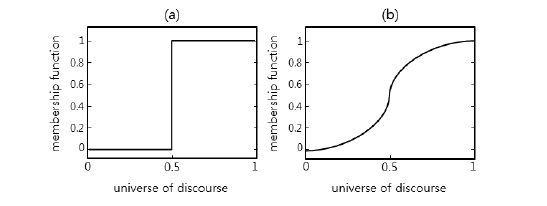
\includegraphics[width=13cm]{Immagini/membfunctcrispvsfuzzy.png}\\
  \caption{Membership function di un crisp set e di un fuzzy set}
  \source{\url{https://bit.ly/3l3O3r6} [Accesso: settembre 2020]}
\end{center}
\end{figure}

In Figura 1.4 è possibile osservare la rappresentazione grafica di un crisp set (a sinistra) e di un fuzzy set (a destra). Il crisp set ha i contorni ben delineati e presenta due soli colori, bianco o nero: ciò accade poiché un punto può o appartenere al set e quindi trovarsi nello spazio in nero, oppure non appartenere al set e dunque trovarsi nello spazio bianco. Il fuzzy set, invece, avrà i contorni più sfumati e zone in grigio, dal momento che contempla l'imprecisione e l'incertezza e pertanto un punto può parzialmente appartenere a un insieme. 

\begin{figure}[h!]
\begin{center}
  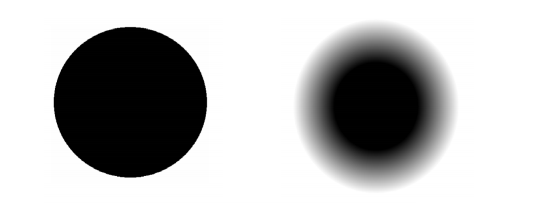
\includegraphics[width=13cm]{Immagini/fuzzyvscrisp.png}\\
  \caption{Rappresentazione grafica di un crisp set e di un fuzzy set}
\end{center}
\end{figure}


% Si può inserire volendo un paragrafo che parla di operazioni su insiemi fuzzy

\subsection{Variabile linguistica e FIS}

Un altro concetto sul quale si basa la logica fuzzy è quello di variabili linguistiche, attraverso cui è possibile avvicinarsi al linguaggio naturale. Infatti, una variabile linguistica ha come valori attributi linguistici, ovvero parole utilizzate nel linguaggio naturale: in particolare, si potranno generare variabili da termini primari (ad esempio ``alto''), modificatori (avverbi come ``molto'', ``sicuramente'', ``abbastanza'' etc.)  e connettori (``e'', ``o'', ``non''). Secondo la definizione di Zadeh, una variabile linguistica viene definita come una quintupla $(V, T(V), U, G, M)$ dove: 

\begin{itemize}
\item $V$ è il nome della variabile linguistica, 
\item $T(V)$ è l'insieme dei termini dei valori linguistici della variabile $V$ (\textit{term set}), 
\item $U$ è l'universo del discorso, cioè il dominio in cui sono definite le variabili, 
\item $G$ è la regola sintattica che genera i nomi in $T(X)$ applicando modificatori linguistici ai termini primari, 
\item $M$ è la regola semantica che assegna a ciascun nome il suo significato, cioè un insieme fuzzy attraverso una funzione di compatibilità $c : U \to [0,1]$. 
\end{itemize}

Ad esempio, data una variabile linguistica $X$ = età, avremo come universo $U$ l'intervallo dei valori assumibili da $X$, ad esempio U=[0, 122]. Un insieme $T(X)$ può essere ''vecchio, molto vecchio, giovane, poco giovane''. La regola $G$ genera nomi applicando modificatori linguistici (``molto'', ``poco'') ai termini primari (``vecchio'', ``giovane''). Infine, la regola $M$ assegnerà ad esempio al valore 27 all'etichetta ``giovane'' con un grado di 0.7. I modificatori, divisi in varie categorie come quelli di concentrazione, di dilatazione e di contrasto, riescono così a rimodellare la regola semantica M, di modo da poter rispecchiare e rappresentare la vaghezza caratterizzante il linguaggio naturale. 

Le variabili linguistiche possono essere utilizzate all'interno dei FIS (\textit{fuzzy inference systems})~\cite{fis}, che consentono il mapping tra input-output crisp attraverso funzioni di appartenenza, operatori logici e regole fuzzy. I FIS vengono utilizzati per classificazione, problemi decisionali, ragionamento approssimativo e altro. Si avvalgono di un processo di fuzzificazione (\textit{fuzzification})~\cite{fuzzific}, cioè di costruzione di un insieme fuzzy a partire da valori di una data variabile, e di defuzzificazione (\textit{defuzzification}), che trasforma un insieme fuzzy in un valore numerico. La fuzzificazione è dunque la fase in cui si determina il grado con cui ogni input appartiene a ogni fuzzy set; per far ciò, ci si avvale della funzione di appartenenza. 

\subsection{Apprendimento automatico supervisionato e fuzzy set}

Per molto tempo, all'interno della teoria dei fuzzy set, grande peso ha assunto la rappresentazione della conoscenza, soprattutto in relazione allo sviluppo di sistemi intelligenti e intelligenza artificiale. Tuttavia, negli ultimi anni sono emersi sempre più problemi con l'approccio puramente \textit{knowledge-driven}, che si basa sull'utilizzo da parte di un sistema di inferenza di conoscenze definite a priori, dal momento che risulta essere difficoltoso, intricato e spesso poco produttivo in termini di risultati. Di conseguenza, si è pensato di adattare i concetti della teoria dei fuzzy set a un approccio \textit{data-driven}, che invece utilizza i dati empirici per estrarre modelli. In questo modo, dunque, si può osservare come la teoria dei fuzzy set sia stata applicata all'interno dell'apprendimento automatico supervisionato, portando così alla nascita della \textit{fuzzy machine learning}~\cite{fuzzyml}. Difatti, la teoria dei fuzzy set riesce a rispondere a problemi di analisi dei dati, risultando pertanto un ottimo strumento per l'ambito dell'apprendimento automatico supervisionato. Difatti, la logica fuzzy risulta idonea, ad esempio, per operare con la vaghezza risultante dai dati empirici, che risentono di linguaggio naturale~\cite{fuzzydata}. 
Gli algoritmi classici del machine learning vengono pertanto estesi ai corrispettivi fuzzy: saranno presenti dunque alberi di decisione fuzzy~\cite{fuzzydectree}, fuzzy clustering~\cite{fcm-intro}, fuzzy k-Nearest Neighbours~\cite{fknn-example1} e così via. In Figura 1.5 è presente un esempio di albero di decisione fuzzy. In questo modo è dunque possibile combinare punti di forza dei metodi classici e della teoria fuzzy al fine di ottenere un metodo che riesce a ottimizzare caratteristiche del modello altrimenti più complessi da migliorare, come l'interpretabilità dei dati e la gradualità. 

\begin{figure}[h!]
\begin{center}
  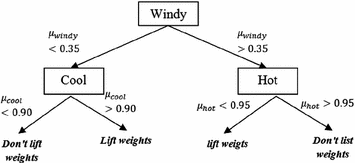
\includegraphics[width=10cm]{Immagini/fuzzyTreeDecis.png}\\
  \caption{Esempio di albero di decisione fuzzy}
\end{center}
\end{figure}

Relativamente al fuzzy machine learning, il focus di questo elaborato è l'induzione di funzioni di appartenenza, cioè la produzione di modelli che, date variabili in input, riescano a predire i gradi di appartenenza a insiemi fuzzy. In generale la costruzione della funzione di appartenenza può essere effettuata attraverso metodi deduttivi e induttivi. I primi sono knowledge-driven, mentre i secondi presentano un approccio data-driven. Nel prossimo capitolo ci si soffermerà su algoritmi induttivi, con il fine di risolvere problemi di classificazione attraverso l'induzione della funzione di appartenenza. 


	\newpage
	\chapter[Tecniche per l'induzione]{Tecniche per l'induzione della funzione di appartenenza}

Generare la funzione di appartenenza è un compito piuttosto complesso all'interno della teoria degli insiemi fuzzy, dovuto all'interpretazione che si può attribuire al concetto di funzione di appartenenza. In particolare, Dubois e Prade~\cite{membinterp} affermano che vi possano essere tre interpretazioni differenti della questione, comportando dunque l'inesistenza di regole generali e sempre ottimali per la generazione della funzione di appartenenza. Ad esempio, la frase ``Il valore di appartenenza di George Bush alla classe di uomini alti è 0.8''~\cite{membpaper} può essere vista in tre differenti modi:

\begin{enumerate}
\item Vista probabilistica: l'80\% della popolazione dichiara che George Bush è alto.
\item Vista dell'insieme casuale: l'80\% della popolazione definisce alto come un intervallo che comprende l'altezza di George Bush.
\item Vista di tipicità: l'altezza di George Bush presenta una distanza normalizzata pari a 0.2 dal prototipo più vicino al concetto di alto, che avrà invece grado di appartenenza pari a 1. 
\end{enumerate}

Non esistendo dunque un'interpretazione univoca, si può ben comprendere come i metodi deduttivi possano risultare inefficaci per stimare la funzione di appartenenza, in quanto uno stesso concetto può essere definito a partire da interpretazioni diverse, ottenendo così diverse funzioni di appartenenza. Non esiste, in altri termini, un processo automatizzabile per la generazione della funzione che risponde perfettamente a ogni situazione proposta. Per ovviare a questo inconveniente, si ricorre agli algoritmi induttivi che consentono di generare la funzione a partire da dati empirici, permettendo dunque di risolvere le ambiguità di interpretazione e di definire maggiormente il dominio. In generale in letteratura sono stati presentati molti algoritmi, tra i quali si annoverano metodi basati sulla percezione, metodi euristici, clustering, support vector machine, istogrammi, k-nearest Neighbour, reti neurali, algoritmi genetici e istogrammi. 
\`E bene notare che non esistono misurazioni che in generale sappiano decretare il metodo migliore per la generazione delle funzioni di appartenenza, ma che questo varia in base al campo e al problema sui quali si opera. Ciò può risultare problematico nel momento in cui si cerca di modellare concetti che non hanno un significato concreto, ma puramente astratto: in tal caso è necessario che il modello utilizzato per indurre la funzione di appartenenza sia abbastanza flessibile e facilmente modificabile, per poterne migliorare le performance generali. La generazione della funzione di appartenenza diviene così un passaggio abbastanza cruciale, dal momento che influenza anche le performance generali dell'algoritmo scelto. La scelta di un metodo a dispetto di un altro risulta dunque fortemente legata al tipo di problema e al tipo di dati ai quali ci si interfaccia. 

In questo capitolo si illustreranno nel Paragrafo 2.1 i metodi basati sulle reti neurali e nel Paragrafo 2.2 i metodi basati sull'algoritmo di k-nearest Neighbour. In entrambi i paragrafi si illustrerà il funzionamento degli algoritmi proposti e si darà una panoramica generale delle possibili varianti. 


	\section{Reti neurali}

Le reti neurali artificiali (ANN) sono modelli computazionali e matematici composti da neuroni artificiali, che traggono ispirazione dalle reti neurali biologiche del cervello umano. Difatti, come le reti neutrali biologiche permettono all'individuo di ragionare e di apprendere, le reti neurali artificiali apprendono attraverso una fitta rete di neuroni interconessi, ognuno dei quali riceve informazioni da alcuni neuroni, le rielabora e spedisce poi il risultato dell'elaborazione ad altri neuroni della rete. Un neurone è una struttura che riceve degli input pesati e contiene una funzione non lineare chiamata funzione di attivazione. In un dato istante, ogni neurone ha un numero memorizzato, che prende il nome di stato. 

Le reti neurali vengono ampiamente utilizzate in molteplici campi, tra cui riconoscimento di pattern (ad esempio in bioinformatica), classificazione e compressione di dati. In questo elaborato, ci si occuperà delle reti feed-forward, dette anche percettroni multistrato, di cui è possibile vedere  un esempio in Figura 2.1. Queste reti neurali presentano essenzialmente tre tipologie di strati o \textit{layer}: un \textit{input layer}, che riceve dati in ingresso, uno o più \textit{hidden layer}, che si occupano dell'elaborazione e un \textit{output layer}, che raccoglie i risultati dell'elaborazione. Il numero di nodi in input è pari al numero delle feature dei vettori di input, mentre il numero di nodi in output è legato alla natura del problema in esame: ad esempio, nei problemi di classificazione binaria si utilizza un solo neurone di output, mentre nei problemi multiclasse il numero di neuroni è pari al numero di etichette considerate.  Ogni neurone in uno strato può avere molteplici connessioni con i neuroni dello strato successivo. Normalmente, si utilizzano strati \textit{fully connected}, in cui ogni neurone è collegato a tutti i neuroni dello strato successivo. 

\begin{figure}[h!]
\begin{center}
  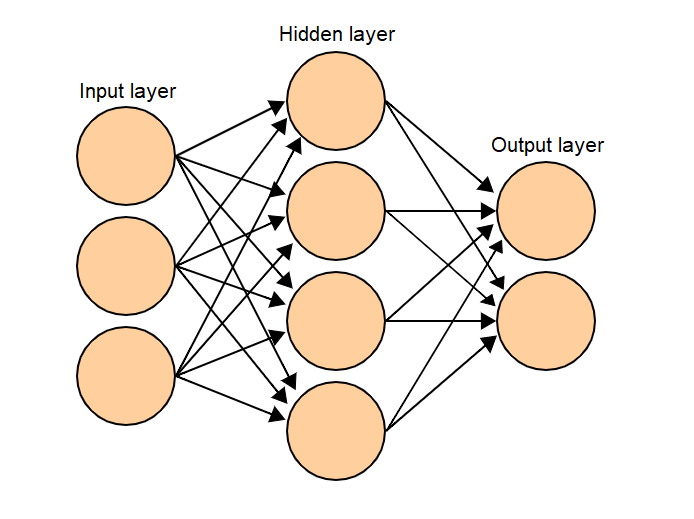
\includegraphics[width=10cm]{Immagini/ReteNeurale.png}\\
  \caption{Struttura di una rete neurale feed-forward}
  \source{\url{https://commons.wikimedia.org/w/index.php?curid=1496812} [Accesso: settembre 2020]}
\end{center}
\end{figure}

Le connessioni tra neuroni presentano dei pesi atti a rafforzare o meno il segnale da mandare al neurone successivo e che vengono aggiustati durante la fase di apprendimento. Spesso, all'interno del neurone vi è una soglia che decreta se tale segnale verrà trasmesso ai neuroni successivi o meno. Per determinare l'output di ogni neurone, si sommano tutti i pesi ricevuti in input, ognuno dei quali è composto dallo stato del neurone del layer precedente moltiplicato per il peso della connessione associata. A questo segnale totale si sottrae l'eventuale soglia del neurone e il risultato finale viene dato in input alla funzione di attivazione che produce il nuovo stato del neurone, che rappresenta anche l'output da trasmettere ai neuroni dello strato successivo. Infine, nell'output layer si raccoglie l'output finale. 

Le reti neurali vengono definite anche ``adattive'', dal momento che sono in grado di modificare i propri pesi attraverso la rielaborazione dei dati esterni e delle informazioni interne, ottenuta durante la fase di apprendimento. Con l'approccio supervisionato, le reti neurali vengono addestrate attraverso esempi, ognuno dei quali è una coppia di input ed etichetta. La rete viene allenata in modo tale che, dato un input, riesca ad approssimare bene l'etichetta corrispondente. Durante il processo di apprendimento, per ogni input fornito, la rete ne predice l'etichetta, che poi confronta con l'etichetta reale corrispondente. La differenza tra output predetto e etichetta corrispondente viene misurata da una funzione di perdita, che diventa l'indicazione per ridefinire i pesi delle connessioni. I pesi delle connessioni, infatti, vengono modificati di modo da minimizzare la funzione di perdita, utilizzando l'algoritmo del gradiente. Per effettuare questa modifica, si procede a ritroso nella rete, partendo dallo strato di output e andando via via a considerare gli strati precedenti, fino ad arrivare a quello di input. Per questo motivo, l'algoritmo di apprendimento viene chiamato backpropagation. 


\subsection{Sistemi neurofuzzy}
Le reti neurali descritte nel paragrafo precedente possono essere utilizzate per generare funzioni di appartenenza, dal momento che i valori di output della funzione di attivazione di ogni neurone possono essere simili ai valori di appartenenza dei fuzzy set~\cite{membneuralnetwsimilar}. Una volta addestrata la rete, pertanto, questa può essere utilizzata per generare gradi di appartenenza, ricevendo in input il vettore delle feature e dando in output il grado di appartenenza ai fuzzy set. Le reti neurali e i fuzzy system hanno delle caratteristiche abbastanza diverse tra loro, come è possibile vedere nella Tabella \ref{table:0}~\cite{neurofuzzyintro}. Entrambi i sistemi presentano i loro punti di forza e le loro debolezze. Da una parte, i sistemi fuzzy sono in grado di rappresentare l'incertezza, sono facilmente estendibili grazie alla generazione di nuove regole e risultano essere robusti, ma sono incapaci di generalizzare. D'altra parte, le reti neurali sanno apprendere e generalizzare, ma è difficile interpretarne il comportamento\footnote{Per questo motivo, una rete neurale viene definita ``scatola nera'', cioè un sistema in cui non sono noti a priori i processi interni che portano al funzionamento del sistema stesso} e determinare il numero di layer e neuroni~\cite{surveyneurofuzzy}.


\begin{table}[h!]
\centering
\begin{tabular}{ |p{7cm}|p{7cm}| } 
\hline
\textbf{Reti neurali} & \textbf{Fuzzy System} \\
\hline
\hline
Sono strutture di basso livello & Affrontano ragionamento di alto livello\\ 
\hline
Buone performance quando si utilizzano molti esempi di apprendimento & Utilizzano informazioni linguistiche da esperti del dominio \\
\hline
Si adattano facilmente a cambiamenti di contesto & Non si adattano facilmente a cambiamenti di contesto \\
\hline
Sono scatole nere per l'utente & Si basano sul linguaggio naturale\\
\hline

\end{tabular}
\caption{Differenze tra reti neurali e fuzzy system}
\label{table:0}
\end{table}

La combinazione di reti neurali e fuzzy system consente di ottenere un sistema capace di integrare la capacità di apprendere delle reti neurali e la flessibilità vicina al ragionamento umano dei sistemi fuzzy. Tale sistema viene detto di tipo \textit{neurofuzzy}, un modello ibrido in cui i due metodi lavorano in modo integrato. Attraverso diverse tecniche delle reti neurali, infatti, è possibile effettuare tuning dei parametri, dei fuzzy set e delle regole all'interno del modello fuzzy. 
Esistono diversi approcci al riguardo, di cui si fornisce una breve elencazione in seguito. 

\begin{itemize}
\item \textit{Cooperative Neuro-Fuzzy System}: esiste una fase di pre-processing in cui attraverso le reti neurali si determinano alcuni sottoblocchi del sistema fuzzy; in seguito, si esegue soltanto il sistema fuzzy. Ha come svantaggio che la struttura diventa non totalmente interpretabile. 
\item \textit{Concurrent Neuro-Fuzzy System}: la rete neurale e il sistema fuzzy lavorano insieme in modo continuativo. Generalmente, l'input entra nel sistema fuzzy, viene pre-processato e in seguito viene immesso nella rete neurale, oppure si può invertire il processo. Uno svantaggio, tuttavia, è la minore interpretabilità dei risultati. 
\item \textit{Hybrid Neuro-Fuzzy System}: la rete neurale apprende alcuni parametri del sistema fuzzy in modo iterativo. Tra tutti è l'approccio più utilizzato. 
\end{itemize}

Nel terzo approccio il sistema complessivo riprende due modalità diverse. Dapprima, nella fase di apprendimento, impara i propri parametri interni come una rete neurale. In seguito, durante la fase di esecuzione, si comporterà come un sistema fuzzy. Questa scelta è stata adottata dal momento che esistono algoritmi efficienti di apprendimento presenti nelle reti neurali, che riescono dunque ad alleviare il processo di tuning dei sistemi fuzzy. Di questo approccio sono state fornite diversi modelli, che spesso risultano essere abbastanza simili tra loro. Una delle famiglie di architetture più comuni è ANFIS (\textit{Adaptive Neuro Fuzzy Inference System}), di cui la Tabella \ref{table:1} indica le principali varianti. 

\subsection{Fuzzy min-max Neural Network}

Negli ultimi anni, la classificazione di pattern è diventata uno dei campi più importanti dell'intelligenza artificiale, dal momento che fornisce innumerevoli applicazioni nel mondo reale. In questo ambito, sia le reti neurali sia la logica fuzzy sono state ampiamente utilizzate, e pertanto si è deciso di costruire un modello ibrido che combina i due sistemi. 
L'algoritmo Fuzzy min-max neural network utilizza i fuzzy set come \textit{pattern class}. L'idea è quella di avere una rete neurale che crea classi aggregando diversi fuzzy set più piccoli in un singolo fuzzy set (fuzzy set class), che corrisponderà alla classe. L'algoritmo si basa sulla costruzione di \textit{hyperbox}. Un hyperbox descrive una regione n-dimensionale definita completamente dai punti di minimo e di massimo, in corrispondenza dei quali viene definita la funzione di appartenenza. In Figura 2.2 è raffigurato un hyperbox, con associata una funzione di appartenenza che determina con quale grado un punto $x\in \mathbb{R}^3$ è contenuto all'interno del box. La collezione di questi hyperbox forma un pattern class. 

\begin{figure}[h!]
\begin{center}
  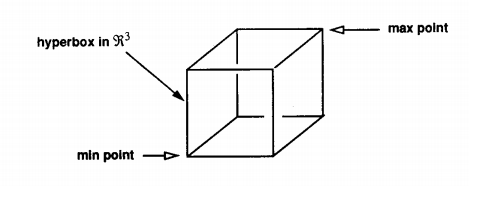
\includegraphics[width=10cm]{Immagini/hyperbox.png}\\
  \caption{Esempio di hyperbox}
\end{center}
\end{figure}

I punti di minimo e di massimo vengono determinati attraverso il \textit{fuzzy min-max learning algorithm}, un processo di espansione e contrazione che impara e definisce i confini dei fuzzy set e quindi delle classi. Ogni fuzzy set class è formato dall'aggregazione di più hyperbox, operazione svolta all'interno della struttura della rete neurale. L'apprendimento avviene collocando correttamente gli hyperbox nel \textit{pattern space}. In seguito è stata fornita una breve descrizione dell'algoritmo fuzzy min-max learning: 

\begin{itemize}
\item espansione: identificare degli hyperbox espandibili ed eventualmente espanderli; se non è possibile trovarne, aggiungere un nuovo hyperbox per la data classe;
\item controllo di sovrapposizioni: determinare se esiste una sovrapposizione di hyperbox tra classi diverse;
\item contrazione: se esiste una sovrapposizione di classi diverse, eliminarla riducendo leggermente ogni hyperbox.
\end{itemize}

In Figura 2.3 è presente un esempio di sovrapposizione. Definiti $v_i$ e $w_i$ rispettivamente il punto minimo e il punto massimo dell'hyperbox i, è possibile notare a sinistra una sovrapposizione tra i due hyperbox che rappresentano classi diverse. Pertanto, occorre effettuare un'operazione di eliminazione, contraendo i confini di ogni hyperbox. 

\begin{figure}[h!]
\begin{center}
  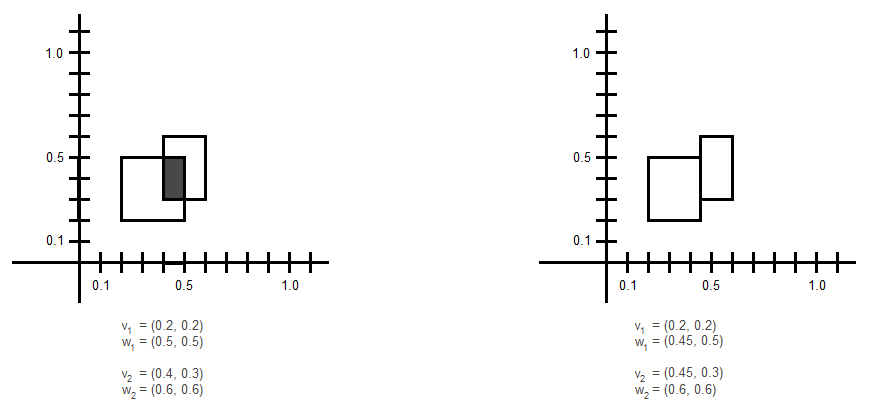
\includegraphics[width=12cm]{Immagini/elimination_overlap.png}\\
  \caption{Esempio di eliminazione di sovrapposizione}
\end{center}
\end{figure}


L'algoritmo fornisce la capacità di incorporare nuove classi e ridefinire quelle esistenti senza dover nuovamente rieffettuare il processo di apprendimento. Tuttavia, presenta anche alcune limitazioni, soprattutto nella procedura di contrazione e controllo di sovrapposizioni, alle quali si è risposto, negli anni, con la presentazione in letteratura di nuove varianti~\cite{fmmnn_variants}. In Figura 2.4 è possibile osservane alcune, principalmente divise tra utilizzo della contrazione o meno. 

\begin{figure}[h!]
\begin{center}
  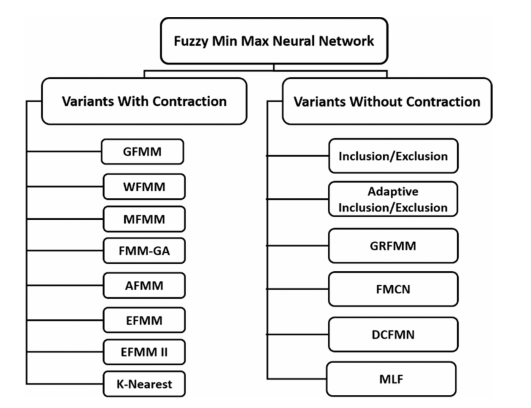
\includegraphics[width=10cm]{Immagini/varianti_FMMNN.png}\\
  \caption{Varianti dell'algoritmo Fuzzy min-max Neural Network}
\end{center}
\end{figure}

Nel Capitolo 3 si vedrà l'implementazione in Python dell'algoritmo Fuzzy min-max Neural Network.

\subsection{Altre varianti}

Infine, oltre ai modelli trattati precedentemente, esistono altre implementazioni di reti neurali fuzzy. Nella Tabella \ref{table:1} è possibile osservare una panoramica di alcuni metodi presenti in letteratura. Per comodità, alcuni metodi sono stati raggruppati per famiglia di algoritmo, di cui è fornita qui in seguito una breve elencazione delle caratteristiche più rilevanti. 

\begin{itemize}
\item \textit{Self-organizing fuzzy neural network}:  capaci di riorganizzare il modello e adattarsi a cambiamenti di \textit{environment}. Si utilizzano nuovi algoritmi di \textit{pruning}, cioè algoritmi di compressione e ottimizzazione della rete neurale. 
\item \textit{Interval Type-2 Fuzzy Neural Network}: estensione con i \textit{Type-2 Fuzzy set}, che consente di esprimere il grado di incertezza per i valori espressi dalla funzione di appartenenza. Presentano una maggiore \textit{learning accuracy} con minor numero di regole rispetto al Type-1.
\item \textit{Dynamic Fuzzy Neural Network}: i neuroni posso essere ricreati o eliminati dinamicamente a seconda delle performance del sistema. L'apprendimento risulta molto più veloce. 
\end{itemize}

Interessante è anche l'algoritmo SVFNN, che combina la maggior capacità nella classificazione da parte delle support vector machine con le potenzialità già elencate delle fuzzy neural network. 


\begin{table}[h!]
\centering
\begin{tabular}{ |c|c|c|c| }
\hline
\textbf{Categoria} & \textbf{Nome metodo} & \textbf{Anno} & \textbf{ Articolo} \\
\hline
\hline
\multirow{3}{17em}{Adaptive neuro fuzzy inference system}  & ANFIS & 1993 & ~\cite{anfis} \\ 
& CANFIS-GA & 2012 & ~\cite{canfi} \\
\hline
\multirow{3}{17em}{Self-organizing fuzzy neural network} & SOFNN & 2004 & ~\cite{sofnn} \\ 
& GenSoFNN & 2002 & ~\cite{gensofnn} \\ 
& SOFNNGA & 2006 & ~\cite{SOFNNGA} \\ 
& SOFNN-IT2 & 2014 & ~\cite{sofnn-it2} \\ 
& GP-FNN & 2010 & ~\cite{GP-FNN} \\
& SOFMLS & 2009 & ~\cite{SOFMLS} \\
\hline
\multirow{3}{17em}{Interval Type-2 Fuzzy Neural Network} & SEIT2FNN & 2008 & ~\cite{SEIT2FNN} \\ 
& IT2FNN  & 2013 & ~\cite{IT2FNN} \\ 
\hline
Fuzzy min-max Neural Networks & FMMNN & 2000& ~\cite{FMMNN}\\	%era il vecchio GFMM
\hline
\multirow{3}{17em}{Dynamic Fuzzy Neural Network} & D-FNN & 2000 & ~\cite{DFNN} \\ 
& GDFNN  & 2001 & ~\cite{GDFNN} \\ 
\hline
Support-Vector-Based Fuzzy Neural Network & SVFNN & 2006 & ~\cite{SVFNN} \\
\hline
Online Self-Constructing  & SONFIN & 1998 & ~\cite{SONFIN} \\
\hline

\end{tabular}
\caption{Elenco degli algoritmi basati su reti neurali}
\label{table:1}
\end{table}

\clearpage


\section{ K-Nearest Neighbour}	
L'algoritmo nearest neighbour è uno degli algoritmi più semplici e facili da implementare nell'apprendimento automatico supervisionato. Vede le sue applicazioni principali nei problemi di classificazione e di regressione. L'idea basilare di questo algoritmo è che due oggetti, se sono simili, saranno vicini tra loro. Si consideri l'insieme $X=\{x_1, x_2, ..., x_n\}$ di $n$ campioni etichettati e si ponga $x_j \in X$ come l'esempio più vicino a un nuovo oggetto $x$. L'algoritmo classificherà $x$ con la stessa etichetta associata a $x_j$. L'algoritmo può essere esteso come  k-Nearest Neighbour, che classifica un oggetto con la stessa etichetta rappresentata dalla maggioranza dei $k$ campioni più vicini. Durante la fase di apprendimento, occorre partizionare lo spazio in diverse regioni, in riferimento alle feature e alle posizioni che occupano gli esempi di apprendimento. Fissato il parametro $k$, corrispondente al numero di vicini necessari per decretare l'etichetta di un oggetto, si andranno a calcolare le distanze tra l'oggetto da classificare e tutti i punti dello spazio, corrispondenti agli esempi di apprendimento. Per calcolare la distanza, dati due punti $ p = (p_1, ..., p_n)$ e $q =  (q_1, ..., q_n)$ si può utilizzare la distanza euclidea:

$$d\left( p,q\right)   = \sqrt {\sum _{i=1}^{n}  \left( q_{i}-p_{i}\right)^2 }$$

\noindent oppure, la distanza di Manhattan: 


$$  d\left( p,q\right) = \sum _{i=1}^{n} \left(|q_{i}-p_{i}|\right)$$


\noindent o, se si opera con stringhe, si può utilizzare la distanza di Hamming. 
Una volta calcolata la distanza tra l'oggetto da classificare e tutti i punti del dataset, le si elencano in ordine non decrescente e si selezionano i primi $k$ punti più vicini. Infine, verrà attribuita all'oggetto l'etichetta più frequente nei $k$ punti più vicini selezionati. 
Un esempio grafico del k-Nearest Neighbour è presente in Figura 2.5. 

\begin{figure}[h!]
\begin{center}
  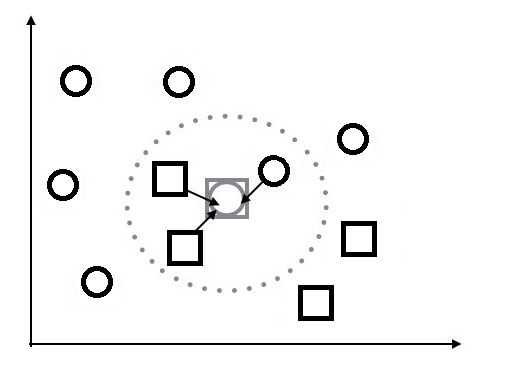
\includegraphics[width=10cm]{Immagini/KNN.png}\\
  \caption{Esempio di k-Nearest Neighbour con $k$ pari a 3}
\end{center}
\end{figure}

Tra i vantaggi di questo algoritmo si possono annoverare la sua estensibilità a molti problemi, l'alta accuratezza e la semplicità di implementazione, e l'adattabilità sui dati. Infatti, l'algoritmo non è parametrico e dunque non viene fatta assunzione sui dati, ma il modello viene costruito interamente dai dati forniti. Tuttavia, l'algoritmo diventa computazionalmente costoso all'aumentare delle dimensioni del dataset, dal momento che conserva la maggior parte dei dati. Ciò comporta tempi cospicui nel dover elaborare un dataset di grandi dimensioni. Un modo per migliorare le performance dell'algoritmo può essere fare \textit{feature selection}, di modo da ridurre il numero di attributi irrilevanti ai fini della classificazione. Un'altra questione delicata è decretare il valore del parametro $k$, in base al quale può variare sensibilmente l'esito della classificazione. Per maggiori chiarimenti si rimanda al Capitolo 3. 

\subsection{Fuzzy k-Nearest Neighbour}

\`E possibile coniugare l'algoritmo k-Nearest Neighbour alla logica fuzzy, ottenendo così il \textit{Fuzzy K-Nearest Neighbour} (FKNN). Questo algoritmo, a differenza della versione base, non assegnerà la classe all'oggetto, ma computerà i gradi di appartenenza a tutte le classi possibili, per evitare nessuna assegnazione arbitraria. I gradi di appartenenza assegnati dipendono dalla distanza dell'oggetto dai k campioni più vicini e dai gradi di appartenenza di quest'ultimi dalle classi possibili. Infatti, uno dei problemi della versione base dell'algoritmo è che i campioni vengono considerati allo stesso modo importanti nell'assegnamento dell'etichetta all'oggetto in questione. Ciò genera spesso difficoltà laddove vi siano sovrapposizioni di campioni. Pertanto, la versione fuzzy  in generale consente di poter definire il grado di appartenenza di un oggetto in una certa classe, in base al quale ridefinire l'importanza dei campioni vicini nel determinare la classe ed evitare situazioni ambigue. Infatti, avere dei gradi di appartenenza permette di poter definire con maggior sicurezza l'appartenenza o meno di un oggetto a una classe e, dunque, consente di aver maggiore sensibilità nella classificazione. Ad esempio, se un oggetto viene assegnato con un grado di appartenenza pari a 0.9 a una classe e 0.05 a un'altra, sarà altamente probabile che l'oggetto appartenga alla prima classe; d'altra parte, se un oggetto ha un grado di appartenenza pari a 0.55 a una classe e un 0.44 a un'altra, allora l'esito della classificazione sarà un po' più incerto. In tal caso allora sarà necessaria maggiore attenzione e magari un secondo esame, per comprendere quale delle due classi sia eventualmente la più consona. Grazie all'implementazione fuzzy, pertanto, si raffina la classificazione. L'algoritmo fuzzy è simile alla versione crisp, dalla quale differisce dopo aver selezionato i $k$ campioni più vicini. 

Nel Capitolo 3 si vedrà l'implementazione in Python del Fuzzy K-Nearest Neighbour. 


\subsection{Varianti}

Il Fuzzy K-Nearest Neighbour presenta alcune debolezze che hanno portato a ricercare varianti per poterle affrontare al meglio. Molte ricerche hanno proposto varie tecniche, tra le quali l'uso della riduzione dei dati, lo sviluppo di metodi per decretare l'iperparametro $k$, l'introduzione dei pesi per adattare l'influenza delle feature e delle versioni più velocizzate per la ricerca dei campioni più vicini. 

In particolare, esiste un'estensione ai fuzzy rough set, che introduce la cosiddetta \textit{classificazione possibilistica}. Infatti, un algoritmo di classificazione dovrebbe notificare la situazione in cui un oggetto non appartiene in realtà a nessuna classe: tale abilità è, difatti, alla base della mente umana, che è in grado di cogliere la non-appartenenza di un oggetto a tutte le classi da lui apprese con l'esperienza. Ad esempio, se un essere umano conosce solo cerchi e rettangoli e gli viene presentato un triangolo, egli sarà in grado di affermare che tale oggetto non apparterrà a nessuna classe da lui conosciuta. L'algoritmo FKNN in generale non possiede questa caratteristica. Si introduce dunque il FRNN, in cui, invece di considerare i $k$ campioni più vicini come punti di riferimento, considera tutti i campioni dello spazio, assegnando gradi di appartenenza diversi. In questo modo, non si presenta il problema di scegliere il valore ottimale di $k$. 

Tra le varianti, è possibile ritrovare nuovamente l'estensione ai Type-2 fuzzy set (si veda il IT2FKNN). Sono presenti anche modalità ibride del FKNN, combinato con algoritmi genetici (GAFuzzyKNN) e clustering (FCMKNN), che consentono di combinare i punti di forza di entrambi gli algoritmi. 

In generale, in Tabella \ref{table:2} è possibile osservare una panoramica di alcuni metodi presenti in letteratura. Per comodità, alcuni metodi sono stati raggruppati per famiglia di algoritmo. Si annoverano le categorie elencate in seguito. 

\begin{itemize}
\item \textit{Interval-valued fuzzy set k-NN}: i valori di membership di ogni campione di training vengono rappresentati come array di intervalli, restituendo una rappresentazione più flessibile della tipicità delle istanze per ogni classe del problema. Usando questo approccio, si riduce sensibilmente la dipendenza al parametro $k$ del FKNN. 
\item \textit{Intuitionistic k-Nearest Neighbour}: utilizzo di intuitionistic set, che sono un'estensione dei fuzzy set classici. Introduce il concetto di grado di non-appartenenza. Sugli esperimenti effettuati, si ottiene un'accuratezza lievemente superiore. 
\item \textit{Possibilistic k-Nearest Neighbour}: introduzione della teoria della possibilità, per gestire in maniera più ottimale rappresentazioni di incertezza. 
\item \textit{Preprocessing Methods via Data Reduction}: lavori di preprocessing al dataset, prima o dopo aver effettuato il processo di training, per diminuire i costi computazionali. Ad esempio, è possibile applicare algoritmi di \textit{pruning}.
\end{itemize}

Infine, un algoritmo recente, molto interessante e che riassume i punti di forza dei metodi presentati in questa tesi è il FNNP, che combina le reti neurali e il FKNN.~\cite{FKNN-NN}

\begin{table}[h!]
\centering
\begin{tabular}{ |c|c|c|c| } 
\hline
\textbf{Categoria} & \textbf{Nome metodo} & \textbf{Anno} & \textbf{Articolo} \\
\hline
\hline
\multirow{3}{17em}{Fuzzy set k-Nearest Neighbour}  & FKNN & 1985 & ~\cite{FKNN} \\ 
& VWFuzzyKNN & 1999 & ~\cite{VWFuzzyKNN} \\
& FCMKNN & 1986 & ~\cite{FCMKNN} \\
& GAFuzzyKNN & 2005 & ~\cite{GAFuzzyKNN} \\
& LPKNN & 2011 & ~\cite{LPKNN} \\
\hline
Fuzzy-rough set k-Nearest Neighbour & FRNN & 2011 & ~\cite{FRNN} \\ 
\hline
\multirow{3}{17em}{Interval-valued fuzzy set k-NN} & IV-kNN  & 2015 & ~\cite{IV-KNN} \\ 
& EF-kNN-IVFS  & 2014 & ~\cite{EF-KNN-IVFS} \\ 
\hline
Type-2 Fuzzy Set k-Nearest Neighbour & IT2FKNN & 2003 & ~\cite{IT2FKNN}\\
\hline
\multirow{3}{17em}{Intuitionistic k-Nearest Neighbour} & IFVKNN & 1998 & ~\cite{IFSKNN} \\ 
& IF-KNN & 1995 & ~\cite{IF-KNN} \\ 
& IFV-NP & 2001 & ~\cite {IF-KNN}\\
\hline
\multirow{3}{17em}{Possibilistic k-Nearest Neighbour} & D-SKNN  & 2002 & ~\cite{D-SKNN} \\ 
& poSIBL  & 2002 & ~\cite{D-SKNN} \\ 
\hline
Modified Fuzzy k-Nearest Neighbour & MOGA-MFNN & 2017 & ~\cite{ MOGA-MFNN} \\
\hline
\multirow{3}{17em}{Preprocessing Methods via Data Reduction} & PFKNN & 2009 & ~\cite{PFKNN} \\
& FuzzyNPC & 1985 & ~\cite{FKNN} \\
& FENN & 1998 & ~\cite{FENN} \\
\hline
Parameter independent fuzzy weighted & PIFW-kNN & 2017 & ~\cite{PIFW-kNN} \\
\hline
\end{tabular}
\caption{Elenco degli algoritmi basati su k-Nearest Neighbour}
\label{table:2}
\end{table}

\clearpage



	\chapter{Implementazioni ed esperimenti}

In questo capitolo si illustrano le implementazioni di due algoritmi, uno per le reti neurali e uno per il k-Nearest Neighbour, trattati nel Capitolo 2. Il codice è disponibile pubblicamente in un repository Github\footnote{https://github.com/ritafolisi/Tirocinio/}. Nel Paragrafo 3.1 si dà una panoramica dei dataset utilizzati, descrivendo le operazioni di preprocessing effettuate. Nei Paragrafi 3.2 e 3.3 si passa in rassegna l'implementazione degli algoritmi Fuzzy min-max Neural Network e Fuzzy k-Nearest Neighbour, illustrati rispettivamente nel Paragrafo 2.1.2 e nel Paragrafo 2.2.1. Si illustra inoltre l'implementazione di alcune tecniche descritte nel Paragrafo 1.1, come la cross-validation e la model selection. Infine, nel Paragrafo 3.4 si discutono i risultati degli esperimenti effettuati. 


	\section{Dataset}
Il primo dataset utilizzato per fare esperimenti è stato Iris, scaricato dal repository UCI Machine Learning\footnote{https://archive.ics.uci.edu/ml/datasets/Iris}. Il dataset, benchmark di base utilizzato nei problemi di classificazione, contiene in totale 150 istanze di iris, classificate in egual numero in tre classi. Ogni classe indica la specie (\textit{Species}) della pianta, ovvero \textit{iris setosa}, \textit{iris virginica} e \textit{iris versicolor}. Per ogni istanza, oltre all'etichetta di classe, viene fornita la dimensione in centimetri della lunghezza (\textit{length}) e larghezza (\textit{width}) del petalo (\textit{petal}) e del sepalo (\textit{sepal}). In Tabella \ref{table:3} sono presenti due esempi di istanze per ogni classe. 

\begin{table} [h!]
    \centering 
    \begin{tabular}{|c|c|c|c|c|}
    \hline
        \textbf{Sepal.lenght} & \textbf{Sepal.width} & \textbf{Petal.length} & \textbf{Petal.width} & \textbf{Species} \\ \hline
        	5.1 	& 3.5 		& 1.4 		& 0.2 		&Setosa\\ 
	4.9 	& 3 		& 1.4 		& 0.2 		&Setosa \\ 
	7.0	& 3.2		& 4.7		&1.4		&Versicolor\\ 
	6.4	& 3.2		& 4.5		&1.5		&Versicolor\\
	6.3	&3.3		&6.0		&2.5		&Virginica\\ 
	5.8	&2.7		&5.1		&1.9		&Virginica\\ \hline	
   \end{tabular}
\caption{Estratto del dataset originale Iris}
\label{table:3}
\end{table}

Come si può osservare, gli attributi sono principalmente quantitativi, tranne Species che presenta invece valori categorici. Nell'apprendimento automatico molti modelli elaborano soltanto quantità numeriche, pertanto è bene convertire le etichette categoriche attraverso un processo che prende il nome di \textit{feature encoding}. Trasformare un valore categorico in uno numerico è in generale un'operazione delicata, in quanto si rischia di creare un ordine tra le classi che, in realtà, non esiste. Nel caso di Iris se si trasformassero le etichette  ``setosa'', ``versicolor'' e ``virginica'' rispettivamente in ``1'', ``2'' e ``3'', potrebbe esserci il rischio che la macchina possa rielaborare una relazione d'ordine tra le tre etichette, che in realtà non sussiste. Esistono molti metodi per effettuare feature encoding. In questo elaborato, si è scelta la classe LabelEncoder, dal package \textit{sklearn.preprocessing}. In questo modo, per ogni etichetta verrà affidato un numero: il dataset quindi avrà come classi ``1'', ``2'' e ``3''. Di questo dataset si è deciso di utilizzare soltanto i primi due attributi (lunghezza e larghezza del sepalo). Inoltre, per visualizzare meglio l'induzione della funzione di appartenenza per ogni classe, a partire da questo dataset ne sono stati generati altri tre. In ognuno di questi, un'etichetta era convertita in 1, mentre le altre erano convertite a 0. Ad esempio, nel dataset ``Iris-setosa'' si pone l'etichetta pari ad ``1'' in corrispondenza di ``setosa'' e a 0 in tutte le altre, e così via. 
In questo modo, data un'istanza, invece di predire a quale delle tre specie appartenesse, si è più interessati se tale istanza sia o meno di una certa specie. 


\begin{table} [h!]
    \centering 
    \begin{tabular}{|c|c|c|c|c|}
    \hline
        \textbf{age} & \textbf{menopause} & \textbf{tumor-size} & \textbf{inv-nodes} & \textbf{node-caps} \\ \hline

	40-49		& premeno		& 15-19		&0-2		&true		\\ 		
	50-59		& ge40		& 15-19		&0-2		&false		\\ 
	50-59		& lt40			& 20-24		&0-2		&NaN		\\ 	
	50-59		& ge40		& 40-44		&3-5		&false		\\ \hline \hline
 \textbf{deg-malig} & \textbf{breast} & \textbf{breast-quad} & \textbf{irradiat} & \textbf{class}\\ \hline 
3		&right		&left\_up	&false		&recurrence-events \\ \
1		&right		&central	&false		&no-recurrence-events \\ 
1		&left		&left\_low	&false		&recurrence-events \\ 
2		&right		&left\_up	&true		&no-recurrence-events \\ \hline		
   \end{tabular}
\caption{Estratto del dataset originale Breast-Cancer}
\label{table:4}
\end{table}

Oltre Iris è stato utilizzato un secondo dataset, per poter analizzare i comportamenti degli algoritmi in esame con un dataset più ampio e più complesso da elaborare. Il dataset scelto è Breast-Cancer, elaborato dall'Istituto di Oncologia dell'University Medical Centre in Lubiana e scaricato dal repository UCI Machine Learning\footnote{https://www.openml.org/d/13}. Il dataset contiene 286 istanze, ognuna delle quali descrive le caratteristiche del tumore al seno e della paziente. Le classi sono ``recurrence-events'' e ``no-recurrence-events'', che si riferiscono al manifestarsi o meno della malattia dopo il trattamento. Oltre all'etichetta, gli attributi sono in totale 9: \textit{age} (età della paziente), \textit{menopause} (se la paziente è in menopausa o meno), \textit{tumor-size} (dimensione del tumore), \textit{inv-nodes} (numero di linfonodi ascellari che contengono carcinoma mammario metastatico), \textit{node-caps} (se il tumore si è infiltrato o meno nella capsula dei linfonodi), \textit{deg-malig} (grado di malignità del tumore), \textit{breast} (se è coinvolto il seno destro o il sinistro), \textit{breast-quad} (localizzazione del tumore) e \textit{irradiat} (se ci si sottopone alla radioterapia). Le istanze sono suddivise in 201 per ``no-recurrence-events'' e 85 per ``recurrence-events''. In Tabella \ref{table:4} sono presenti due esempi di istanze per ogni classe. 

Anche in questo caso ci sono attributi categorici, come breast o irradiat, che saranno poi convertiti in quantitativi con LabelEncoder. Alcuni attributi, come tumor-size, sono esplicitati attraverso intervalli di valori: in questo caso si è deciso di considerarne solo il punto medio. Il dataset originale presenta anche dei valori mancanti (indicati tramite NaN in Tabella \ref{table:4}) e alcuni duplicati, che sono stati entrambi rimossi. Dopo questa operazione di preprocessing, la dimensione finale del dataset  è 263 elementi, di cui 77 con etichetta ``recurrence-events'' e 186 con ``no-recurrence-events''. 


	\section{Fuzzy min-max Neural Network}
In questo paragrafo si presenta l'implementazione del Fuzzy min-max Neural Network, di cui è stato dato un accenno nel capitolo precedente. Il punto di partenza è stato un codice scaricato da un repository pubblico\footnote{https://github.com/Cartmanishere/fuzzy-min-max-classifier}, che successivamente è stato adattato e sistemato secondo le esigenze del tirocinio. Nel file \textit{fuzzy.py} del repository del tirocinio, è possibile vedere l'algoritmo Fuzzy min-max, configurato sottoforma di classe. 

Questa implementazione è stata utilizzata per vari esperimenti durante il tirocinio. Inizialmente è stato adottato un approccio esplorativo utilizzando un notebook Jupyter. In seguito, è stato estratto uno script che permettesse l'esecuzione automatizzata di esperimenti, specificando il dataset tramite argomenti nella linea di comando. Nel repository del tirocinio, questo script viene poi richiamato da un altro script, \textit{final\_script.py}, che riceve in argomento da linea di comando il dataset e l'algoritmo da utilizzare per effettuare esperimenti. Nel file \textit {unittest\_fmm.py} sono stati effettuati unit test per controllare il buon funzionamento del codice scritto. In particolare, sono state verificate le principali funzionalità del modello, l'ammissibilità dei valori restituiti dalle metriche e il fatto che l'RMSE fosse sotto una soglia accettabile. 

In ogni esperimento è prevista una cross-validation annidata, per poter effettuare anche il tuning degli iperparametri della rete. Per poter effettuare questa cross-validation, è stata utilizzata la classe \textit{StratifiedKFold} dal package \textit{sklearn.model\_selection}. Si avrà dunque una cross-validation esterna che divide i dati in $k$ fold e per ogni fold $i$ = 1, ..., $k$ si effettua una cross-validation interna, che elabora tutti i fold tranne l'$i$-esimo. All'interno della cross-validation interna viene effettuata la model selection: i dati risultanti vengono divisi ulteriormente in $l$ fold e per ogni configurazione di iperparametri, per ogni $j$ = 1, ..., $l$ si addestra un modello utilizzando tutti i fold tranne il $j$-esimo, e lo si valuta sul fold $j$-esimo. Per la model selection è stata utilizzata la libreria \textit{GridSearchCV}, che opera costruendo una griglia contenente i validation score ottenuti dal modello, allenato di volta in volta con ogni possibile configurazione degli iperparametri. In questo caso, il validation score coincide con l'accuratezza. Per poter utilizzare GridSearchCV è necessario che il modello rispetti l'interfaccia di sklearn, ovvero implementare una serie di metodi, tra cui score, predict, fit, get\_params e set\_params. Nell'implementazione originale non erano presenti i metodi get\_params e set\_params, che sono stati opportunamente definiti in seguito: il primo consente di restituire i parametri da ottimizzare e il secondo di modificarli. Gli iperparametri da ottimizzare, in questo caso, sono la sensitivity, di cui si parlerà in seguito, ed \textit{exp\_bound}, pari al limite dell'espansione di un hyperbox. Per entrambi, la selezione avviene considerando i valori \{0 , 0.1, 0.2, 0.3, 0.4, 0.5, 0.6, 0.7, 0.8, 0.9, 1\}. Al termine della cross-validation interna, pertanto, si ottiene un modello, che viene poi valutato sull'$i$-esimo fold. Negli esperimenti, il numero di fold per la cross-validation interna ed esterna è stato fissato a cinque. Ogni valutazione effettuata all'interno della cross-validation esterna è stata memorizzata in un array. Le metriche utilizzate in questo caso sono state l'accuratezza e l'RMSE tra l'etichetta dell'input e la membership indotta dal modello. I metodi che restituiscono questi valori sono stati opportunamente implementati durante il tirocinio. 


Questo algoritmo viene utilizzato particolarmente nei problemi di classificazione. Si consideri in generale come input un vettore n-dimensionale $A_h$, che viene immesso in $k$ funzioni discriminanti, ognuna delle quali calcola un punteggio per la propria classe, compreso tra 0 e 1. Si seleziona la funzione che restituisce il valore più alto e si assegna l'input a quella classe. In modo analogo questo meccanismo può essere esteso al campo fuzzy: al posto delle funzioni discriminanti si utilizzano $k$ funzioni di appartenenza, ognuna delle quali si riferisce a un fuzzy set. Ogni fuzzy set fa riferimento a una classe alla quale un input può appartenere, ed è formato dall'aggregazione di fuzzy set più piccoli. Per distinguere i due tipi di insiemi, ci si riferisce al primo come \textit{fuzzy set class}. In Figura 3.1 è raffigurata la struttura di un sistema che classifica pattern. 

\begin{figure}[h!]
\begin{center}
  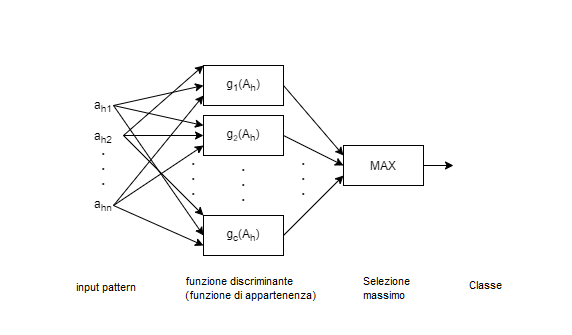
\includegraphics[width=12cm]{Immagini/FMMNN_nn.png}\\
  \caption{Sistema per la classificazione di pattern}
\end{center}
\end{figure}

I fuzzy set vengono rappresentati come hyperbox, già trattati nel capitolo precedente. Dato un hyperbox $B_j$, la classe $k$-esima $C_k$ viene definita come
$$ C_k = \bigcup_{j \in k} B_j $$
\noindent dove $j$ indica l'indice di tutti gli hyperbox associati alla classe $k$. %Nella teoria dei fuzzy set, l'unione tra più fuzzy set coincide con il massimo delle funzioni di appartenenza. 
Dato in input un vettore $A_h$, la funzione di appartenenza  al $j$-esimo hyperbox viene indicata con $b_j(A_h)$ ed è pari ad 1 in caso di piena appartenenza, altrimenti diminuisce all'aumentare della distanza tra i punti del vettore, secondo la seguente formula: 

\begin{equation} \label{eq:1}
\begin{split}
 b_j (A_h) = {1 \over 2n} \sum_{i=1}^n [\max (0.1-\max (0, \gamma \min (1, a_{hi} - w_{ji}))) \\
+ \max(0.1-\max(0, \gamma \min(1, v_{ji} - a_{hi})))]
\end{split}
\end{equation}

\noindent dove $\gamma$ è la sensibilità (\textit{sensitivity}), un iperparametro della rete che indica quanto deve diminuire il valore della funzione di appartenenza all'aumentare della distanza tra $A_h$ e $B_j$. I vettori $W$ e $V$ indicano rispettivamente i punti di massimo e i punti di minimo dell'hyperbox $B_j$; infine, $n$ indica la dimensione del vettore $A_h$. 

In questo tirocinio l'algoritmo fuzzy min-max è stato implementato con una rete neurale, per ottenere maggiore velocità ed efficienza. In Figura 3.2 è presente l'architettura generale della rete neurale, divisa in tre strati. 


\begin{figure}[h!]
\begin{center}
  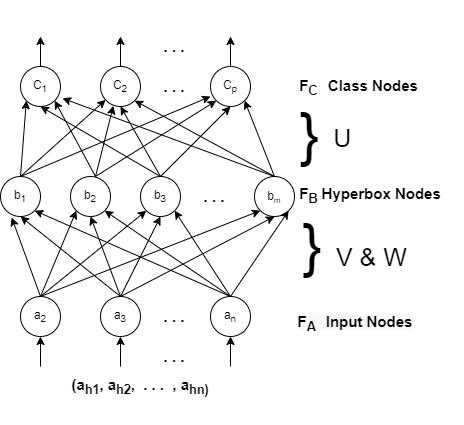
\includegraphics[width=10cm]{Immagini/architecture_FMMNN.png}\\
  \caption{Struttura di una rete neurale che implementa fuzzy min-max}
\end{center}
\end{figure}

Il primo strato è quello di input, $F_A$, che contiene gli $n$ elementi del vettore in input $A_h$. Questo strato è connesso al secondo, $F_B$, che rappresenta gli hyperbox. Per determinare le connessioni tra questi stati, si ricorre a (\ref{eq:1}), utilizzando i vettori $V$ e $W$ che contengono i punti di minimo e di massimo. I pesi di queste connessioni vengono aggiornati durante il processo di apprendimento della rete neurale, attraverso l'algoritmo fuzzy min-max learning, già visto nel capitolo precedente. Lo strato degli hyperbox è connesso a quello delle classi, $F_C$, con valori binari memorizzati in una matrice $U$, in cui ogni elemento viene così calcolato: 

$$ u_{jk} = \bigg \{ 
\begin{array}{rl}
1 &\text{se } b_j \text{ è hyperbox per la classe } c_k \\
0 & \text{altrimenti} \\
\end{array}
$$

\noindent dove $b_j$ è il $j$-esimo nodo dello strato $ F_B$ e  $c_k$ è il $k$-esimo nodo dello strato $ F_C$. Ogni nodo in $F_C$ rappresenta una classe e fornisce in output il grado con cui l'input $A_h$ appartiene alla propria classe. Per determinarlo, si seleziona il massimo valore di appartenenza tra gli hyperbox della classe: i valori di hyperbox di altre classi non sono considerati. In formule, si ha: 

$$ c_k = max_{j = 1, \dots, m} b_j u_{jk} $$

Pertanto se l'hyperbox j non appartiene alla classe k, avrà $u_{jk} $ pari a zero e il suo valore $b_j$ risulterà irrilevante. 
In Figura \ref{fmm_hyperbox} è possibile osservare gli hyperbox creati durante il processo di apprendimento del dataset iris-versicolor. 

\begin{figure}[h!]
\begin{center}
  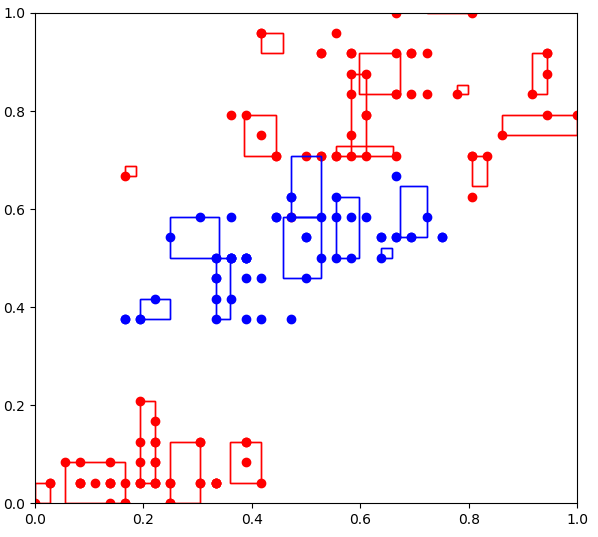
\includegraphics[width=10cm]{Immagini/hyperbox_created_irisversicolor.png}\\
  \caption{hyperbox creati con iris-versicolor}
  \label{fmm_hyperbox}
\end{center}
\end{figure}



	\section{Fuzzy k-Nearest Neighbour}


In questo paragrafo è presentata l'implementazione dell'algoritmo Fuzzy k-Nearest Neighbour, di cui è stato dato un accenno nel capitolo precedente. Il punto di partenza è stato un codice scaricato da un repository pubblico\footnote{https://github.com/sahilsehwag/FuzzyKNN}, che in seguito è stato adattato e sistemato secondo le esigenze del tirocinio. All'interno del repository del tirocinio, il codice dell'algoritmo è reperibile nel file \textit{fknn.py}. È stato adottato anche in questo caso un primo approccio esplorativo, utilizzando un notebook Jupyter. Successivamente, è stato estratto uno script per automatizzare l'esecuzione degli esperimenti, specificando il dataset come argomento nella linea di comando. Questo script viene poi richiamato da \textit{final\_script.py}, già descritto precedentemente. Negli esperimenti proposti, le metriche di valutazione adottate sono del tutto analoghe con quelle presentate nel paragrafo precedente. Anche in questo caso si restituiscono l'accuratezza e l'RMSE tra etichetta e grado di appartenenza indotto.  Infine, nel file \textit{unittest\_fknn.py} sono stati effettuati unit test sul codice, per verificare la correttezza delle principali funzionalità in maniera del tutto analoga al Fuzzy min-max. 


Come già descritto nel capitolo precedente, questo algoritmo è molto simile all'implementazione crisp, ma grazie all'introduzione di grado di appartenenza consente di raffinare la classificazione. I dati di apprendimento sono vettori n-dimensionali e nella fase di training vengono semplicemente memorizzati, suddividendoli ognuno in vettore delle feature e vettore di classe. Prima della fase di classificazione, bisogna fissare l'iperparametro $k$. Questo iperparametro regola quanti vicini bisogna considerare per predire il grado di appartenenza di un input $x$ e pertanto può alterare sensibilmente i risultati della classificazione. Quando $k$ è pari ad 1, allora la classificazione viene effettuata considerando un solo vicino, con il rischio di una pessima classificazione qualora ci sia rumore nei dati di apprendimento: infatti, in tal caso si predirebbe un'etichetta erronea per $x$. D'altra parte, se si ponesse $k$ pari al numero totale dei dati di apprendimento, si perderebbe il senso dell'algoritmo e l'input verrebbe semplicemente classificato con l'etichetta che compare con maggior frequenza all'interno del dataset. Riassumendo, dunque, se $k$ assumesse un valore alto, si registrerebbe maggiore precisione nella classificiazione; ma d'altra parte, se $k$ assume un valore troppo grande, il processo di classificazione potrebbe diventare poco chiaro o, peggio, facilmente deducibile a priori. Altri due criteri che possono incidere nella scelta dell'iperparametro $k$  sono eventuali sovrapposizioni di classe, a causa delle quali un vicino può appartenere a più di una classe, o la presenza di molto rumore nel dataset. In generale è consigliabile, prima di procedere con l'algoritmo, effettuare operazioni di preprocessing. Alla luce di quanto detto, è evidente che la scelta di $k$ deve tener conto di molti aspetti. Definire a priori un $k$ corretto, che vada bene sempre, è un'operazione impossibile: è necessario dunque analizzare ogni caso singolarmente. A tal proposito, per decretare il valore di $k$ è utile fare una model selection, con le stesse modalità già descritte nel paragrafo precedente. Gli esperimenti effettuati, dunque, avranno la stessa struttura vista con il Fuzzy min-max: si utilizza una cross-validation annidata e quella interna si occuperà della model selection. Anche in questo caso si lavora con StratifiedKFold e GridSearchCV, dunque è necessario adattare l'implementazione del Fuzzy k-Nearest Neighbour all'interfaccia di sklearn, aggiungendo i metodi get\_params e set\_params. Nel codice originale i valori di $k$ considerati sono i valori dispari compresi tra 1 e 19. 

Fissato $k$, è possibile iniziare il processo di predizione dell'etichetta per l'input $x$. Innanzitutto, si calcola la distanza tra ogni punto del dataset e $x$ e si selezionano i $k$ punti più vicini. In seguito, per ogni classe $i$ si calcola la funzione di appartenenza $u_{i}(x)$, nel seguente modo: 

\begin{equation} \label{eq:2}
u_{i}(x) = {\sum_{j=1}^k u_{ij}({1 / \Vert x-x_j\Vert^{\frac{2}{m-1}}}) \over \sum_{j=1}^k ({1 / \Vert x-x_j\Vert^{\frac{2}{m-1}}}) }
\end{equation}

\noindent dove $u_{ij}$ è il grado di appartenenza del vicino $j$ appartenente alla classe $i$. La costante $m$ determina quanto bisogna pesare la distanza quando si calcola il contributo di ogni vicino al grado di appartenenza di $x$. Nell'implementazione effettuata, $m$ è stato posto pari a due, pertanto il contributo di ogni vicino è ponderato dal reciproco della distanza euclidea da $x$. La classe che ottiene il grado di appartenenza maggiore sarà l'etichetta predetta per $x$. Può succedere che $x$ coincida con un vicino $x_j$. In tal caso si ha che $u_i(x) = u_i(x_j) $, cioè il grado di appartenenza alla classe $i$ del punto $x$ è pari al grado di appartenenza del vicino $x_j$. Non essendo stata gestita questa situazione nel codice originale, durante i primi esperimenti succedeva che i gradi di membership indotti assumessero valori pari ad infinito, causando così problemi nel valutare le performance. Questo problema è stato opportunamente risolto correggendo il metodo predict. 


	\section{Risultati}


In questo paragrafo si illustreranno i risultati ottenuti dagli esperimenti effettuati. Sono stati utilizzati file di log per registrare le accuratezze e l'RMSE, oltre che per avere un'indicazione generale della durata che ogni algoritmo impiega per elaborare i dati ed effettuare le predizioni. In Tabella \ref{table:exper} è possibile vedere i risultati ottenuti con il Fuzzy min-max. 

Il metodo in generale predice bene i dati, ottenendo accuratezze abbastanza elevate rispetto agli altri metodi considerati. Tuttavia, l'RMSE tra etichetta e grado di appartenenza indotto risulta essere abbastanza alto, in relazione all'accuratezza. Con il dataset Iris-setosa, ad esempio, benché ci sia un'accuratezza pari al 99\% si ha un errore pari a 0.64. Per visualizzare meglio il problema, si osservino le proiezioni delle curve di livello dei gradi di appartenenza in Figura \ref{curvegfmm} e le relative heatmap in Figura \ref{heatmapgfmm}. 
Dai grafici è possibile notare che i gradi di appartenenza indotti sono in generale abbastanza alti, senza alcuna distinzione tra classi. Ciò rappresenta un punto debole dell'algoritmo, dal momento che la classificazione, seppur con una buona accuratezza, non risulta totalmente precisa. 


\begin{figure}[h!]
		\centering
		\subfloat[\emph{}]
		{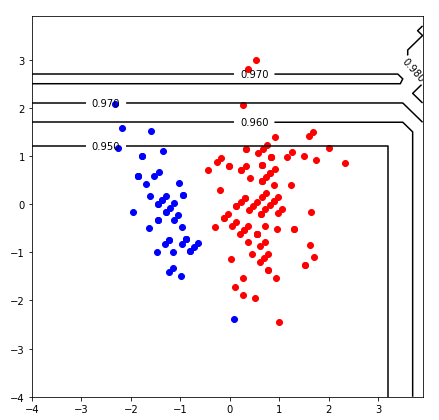
\includegraphics[width=.44\textwidth]{Immagini/GFMM_setosa.png}} 
		\quad
		\subfloat[\emph{}]
		{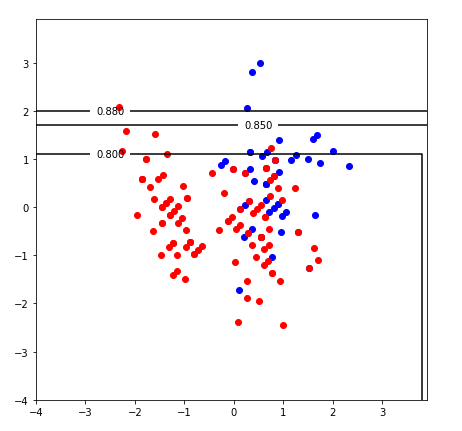
\includegraphics[width=.46\textwidth]{Immagini/GFMM_virginica.png}} \quad
		\subfloat[\emph{}]
		{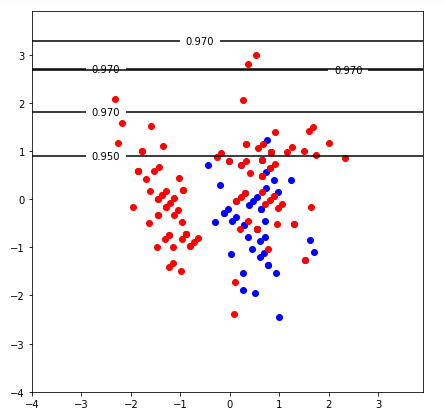
\includegraphics[width=.45\textwidth]{Immagini/GFMM_versicolor.png}} \quad
		\caption{Curve di livello con Fuzzy min-max: (a) setosa, (b) virginica, (c) versicolor}
		\label{curvegfmm}
	\end{figure}	


\begin{figure}[h!]
		\centering
		\subfloat[\emph{}]
		{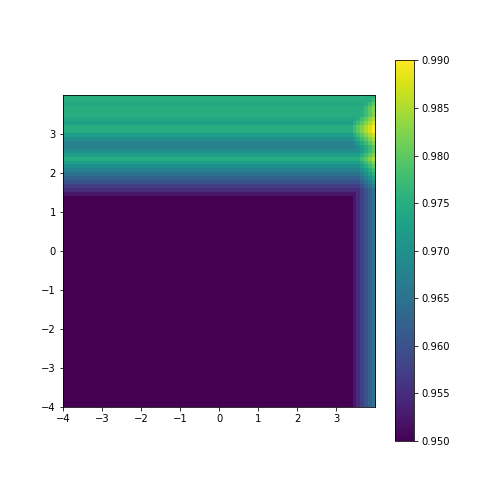
\includegraphics[width=.44\textwidth]{Immagini/gfmm-set-hm.png}} 
		\quad
		\subfloat[\emph{}]
		{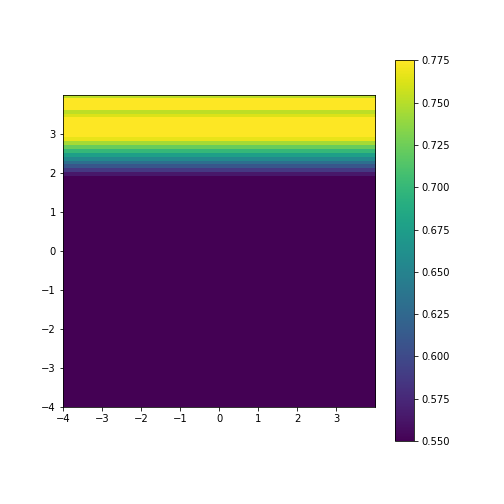
\includegraphics[width=.44\textwidth]{Immagini/gfmm-virg-hm.png}} \quad
		\subfloat[\emph{}]
		{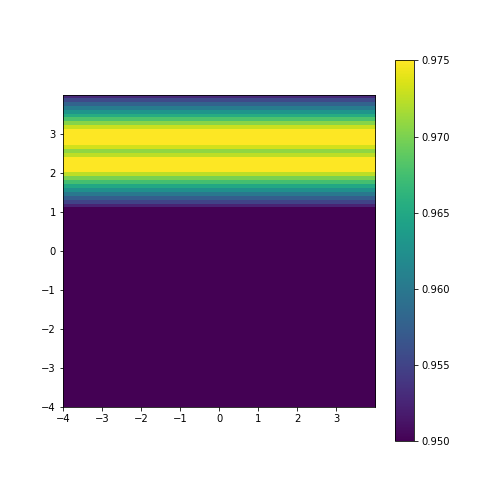
\includegraphics[width=.44\textwidth]{Immagini/gfmm-vers-hm.png}} \quad
		\caption{Heatmap con Fuzzy min-max: (a) setosa, (b) virginica, (c) versicolor}
		\label{heatmapgfmm}
	\end{figure}	



In Tabella \ref{table:exper} sono riportati i risultati ottenuti dagli esperimenti con il Fuzzy k-Nearest Neighbour. 
Le accuratezze in generale sono vicine a quelle osservate nel Fuzzy min-max, con valori sensibilmente inferiori per l'RMSE tra etichetta e grado di membership indotto. Iris-setosa viene predetto con un'accuratezza pari al 99\% e ha un RMSE pari a 0.08, il che risulta coerente. Performance peggiori sono state rilevate però con il dataset Breast-Cancer, dove invece si comporta decisamente meglio il Fuzzy min-max. Partendo dallo stesso problema di classificazione, il Fuzzy k-Nearest Neighbour impiega molto più tempo per effettuare predizioni (circa 9 minuti) rispetto al Fuzzy min-max (un minuto e mezzo). Per migliorare le tempistiche potrebbe essere utile effettuare operazioni di preprocessing sui dati, quali la feature selection, riduzione di rumore e la normalizzazione.



Infine, sono riportati in Tabella \ref{table:exper} i risultati degli algoritmi Fuzzy C-means e Support Vector Machine - Class Imbalance Learning\footnote{In Tabella \ref{table:exper} non è presente l'errore RMSE in quanto non è stato possibile estrarre i gradi di appartenenza}, implementati in un elaborato affine a questo, ma che si soffermava su clustering e support vector machine~\cite{bib:alessia}. 


\begin{table}[h!]
\centering
\begin{tabular}{ |c|c|c|c| } 
\hline
\textbf{Algoritmo} & \textbf{Dataset} & \textbf{Accuratezza} & \textbf{RMSE} \\
\hline
\hline
\multirow{3}{14em}{Fuzzy min-max}  & Iris-setosa & 99\% & 0.64 \\
& Iris-versicolor & 76\% & 0.63 \\
& Iris-virginica & 78\% & 0.57 \\
& Breast Cancer Dataset & 71\%  & 0.84 \\
\hline
\multirow{3}{14em}{Fuzzy k-Nearest Neighbour} &  Iris-setosa & 99\% & 0.08 \\
& Iris-versicolor & 76\% & 0.44 \\
& Iris-virginica & 75\% & 0.44 \\
& Breast Cancer Dataset & 62\% & 4.6 \\             
\hline
\multirow{3}{14em}{Fuzzy C-means}  & Iris-setosa & 98\% & 0.12\\
&Iris-versicolor & 64.7\% & 0.55\\
& Iris-virginica & 68.7\% & 0.69\\
& Breast Cancer Dataset &  56.2\% & 0.54\\
\hline
\multirow{3}{14em}{Fuzzy SVM-CIL}  & Iris-setosa & 100\% & - \\
& Iris-versicolor & 94\% & - \\
& Iris-virginica & 96.7\% & - \\
& Breast Cancer Dataset &  72.6\% & - \\
\hline
\end{tabular}
\caption{Risultati degli esperimenti}
\label{table:exper}
\end{table}



	\chapter*{Conclusioni}

In questo elaborato ci si è focalizzati sulla ricerca, la modifica e il riuso di algoritmi per l'induzione della funzione di appartenenza a insiemi fuzzy. Sono stati introdotti i concetti principali legati all'apprendimento automatico e agli insiemi fuzzy, illustrando questi come possano essere coniugati per gestire l'ambiguità del linguaggio naturale. In seguito, ci si è soffermati sul significato dell'induzione di una funzione di appartenenza, elencando le modalità con cui si può effettuare. Sono stati utilizzati algoritmi basati sulle reti neurali e sul k-Nearest Neighbour. In particolare, si sono viste le implementazioni del Fuzzy min-max Neural Network e del k-Nearest Neighbour. Per entrambi gli algoritmi, partendo da codice preesistente, sono state aggiunte funzionalità e attuate modifiche per consentire la realizzazione di esperimenti in modo armonizzato. Al termine degli esperimenti, sono state raccolte le valutazioni delle prestazioni, espresse in tabelle e grafici. Sui dataset proposti, Iris e Breast-Cancer, Fuzzy min-max ha raggiunto un'accuratezza maggiore per quanto riguarda il processo di classificazione, impiegando meno tempo per effettuare elaborazione sui dati e predizioni. D'altra parte, Fuzzy k-Nearest Neighbour ha conseguito un errore minore nell'indurre i gradi di appartenenza. 

Questo lavoro può essere ulteriormente sviluppato prendendo in considerazione nuovi algoritmi o nuovi dataset più complessi da elaborare, di modo da poter estendere il confronto a nuove proposte. In tal caso, durante il tirocinio, è stato impostato il framework da utilizzare come base di partenza.


\bibliographystyle{ieeetr}
\bibliography{bibliografia}

\end{document}